\documentclass[11pt,letterpaper]{book}
\usepackage[latin1]{inputenc}
\usepackage[margin=.75in]{geometry}
\usepackage{amsmath}
\usepackage{amsfonts}
\usepackage{amssymb}
\usepackage{graphicx}
\usepackage{textcomp}
\usepackage{multirow}
\usepackage{rotating} 
\usepackage{hyperref}
\usepackage{multicol}
\usepackage{scalefnt}
\usepackage{datetime}
\usepackage[toc,lof]{multitoc}
\hypersetup{
    %bookmarks=true,         % show bookmarks bar?
    unicode=false,          % non-Latin characters in Acrobat’s bookmarks
    pdftoolbar=true,        % show Acrobat’s toolbar?
    pdfmenubar=true,        % show Acrobat’s menu?
    pdffitwindow=false,     % window fit to page when opened
    pdfstartview={FitH},    % fits the width of the page to the window
    pdftitle={py[xlr8r] User Reference Notes},    % title
    pdfauthor={Bruce E Shapiro},     % author
    pdfsubject={py[cellerator], pycellerator,  cellerator, python, ipython},   % subject of the document
    pdfcreator={Math 370},   % creator of the document
    pdfproducer={PDFLaTeX}, % producer of the document
    pdfkeywords={py[cellerator], pycellerator, cellerator}, % list of keywords
    pdfnewwindow=true,      % links in new window
    colorlinks=true,       % false: boxed links; true: colored links
    linkcolor=blue,          % color of internal links
    citecolor=green,        % color of links to bibliography
    filecolor=magenta,      % color of file links
    urlcolor=blue           % color of external links
}
\title{

\includegraphics[width=\textwidth]{pycellerator-logo.png}
}
\author{\Huge{Reference Notes}}
\date{\href{mailto:bruce.e.shapiro@csun.edu}{bruce.e.shapiro@csun.edu} \\ Department of Mathematics\\California State University, Northridge\\\vspace{2ex}Revised: \today\ at \currenttime}


\newcommand{\LJ}[1]{{
\begin{minipage}{1in}
\begin{flushleft}\textbf{#1}\end{flushleft}
\end{minipage}
}}
\newcommand{\LM}[1]{{
\begin{minipage}{2in}
\begin{flushleft}{#1}\end{flushleft}
\end{minipage}
}}
\newcommand{\LMM}[1]{{
\begin{minipage}{3in}
\begin{flushleft}{#1}\end{flushleft}
\end{minipage}
}}
\newcommand{\TT}[1]{\ensuremath{\text{\tt{#1}}}}
\newcommand{\TTI}[1]{\TT{\textit{#1}}}


\usepackage{fancyvrb}

\newcommand{\SW}[1]{\begin{sideways}{#1}\end{sideways}}

\newenvironment{changemargin}[2]{%
  \begin{list}{}{%
    \setlength{\topsep}{0pt}%
    \setlength{\leftmargin}{#1}%
    \setlength{\rightmargin}{#2}%
    \setlength{\listparindent}{\parindent}%
    \setlength{\itemindent}{\parindent}%
    \setlength{\parsep}{\parskip}%
  }%
  \item[]}{\end{list}}

\setlength{\parindent}{0pt}
\setlength{\parskip}{1ex}


\usepackage[usenames,divnames,svgnames,dvinames]{xcolor,colortbl}

\definecolor{pygray}{RGB}{204,255,229} % really its light green
\newcommand{\GRAY}{\cellcolor{pygray}}

\usepackage{listings}

\usepackage{pdfpages}
%
% the following changes the selection of the ttfont
% the default is cmtt (computer modern font), which does not have a bold face
% replace it with pcr (courier font)
\renewcommand{\ttdefault}{pcr}
\lstset{
	language=Python,
	basicstyle=\normalfont\ttfamily\small\bfseries,
	keywordstyle=\ttfamily\bfseries,
	frame=single,
	backgroundcolor=\color{pygray},
	escapeinside={//*}{*//},
	xleftmargin=.375in,
	xrightmargin=.375in,
	showstringspaces=false % turn off squat-u for strings
	}


\newcommand{\CODE}[1]{{\small {\tt \textbf{#1}}}}
\newcommand{\FCODE}[1]{{\footnotesize {\tt \textbf{#1}}}}


\begin{document}

\frontmatter

\maketitle

\copyright \ 2015 Bruce E Shapiro \\ \vspace{-8pt} \hrule
\begin{small}
This work is licensed under the Creative Commons Attribution-NonCommercial-NoDerivs 3.0 United States License. To view a copy of this license, visit \url{http://creativecommons.org/licenses/by-nc-nd/3.0/us/}  or send a letter to Creative Commons, 444 Castro Street, Suite 900, Mountain View, California, 94041, USA.\\
The following is a summary of the license.  

You are free:
\vspace{-12pt}
\begin{itemize}
\item to Share -- to copy, distribute and transmit the work
\end{itemize}
\vspace{-12pt}
Under the following conditions:
\vspace{-12pt}
\begin{itemize}
\setlength{\itemsep}{0pt}
\setlength{\parsep}{0pt}
\setlength{\topsep}{0pt}
\setlength{\parskip}{0pt}
\setlength{\partopsep}{0pt}
\item Attribution -- You must attribute the work in the manner specified by the author or licensor (but not in any way that suggests that they endorse you or your use of the work).
\item Noncommercial -- You may not use this work for commercial purposes.
\item No Derivative Works -- You may not alter, transform, or build upon this work.
\end{itemize}
\vspace{-12pt}
With the understanding that:
\vspace{-12pt}
\begin{itemize}
\setlength{\itemsep}{0pt}
\setlength{\parsep}{0pt}
\setlength{\topsep}{0pt}
\setlength{\parskip}{0pt}
\item Waiver -- Any of the above conditions can be waived if you get permission from the copyright holder.
\item Public Domain -- Where the work or any of its elements is in the public domain under applicable law, that status is in no way affected by the license.
\item Other Rights -- In no way are any of the following rights affected by the license:
\vspace{-4pt}
\begin{itemize}
\setlength{\itemsep}{0pt}
\setlength{\parsep}{0pt}
\setlength{\topsep}{0pt}
\setlength{\parskip}{0pt}
\item Your fair dealing or fair use rights, or other applicable copyright exceptions and limitations;
\item The author's moral rights;
\item Rights other persons may have either in the work itself or in how the work is used, such as publicity or privacy rights.
\end{itemize}
\end{itemize}
\vspace{-12pt} 
Notice -- For any reuse or distribution, you must make clear to others the license terms of this work. The best way to do this is with a link to the web page \url{http://creativecommons.org/licenses/by-nc-nd/3.0/us/}. \\
\hrule
Figure 1.2 is licensed subject to CC-BY-SA 3.0 and GPL 2.0. 

\hrule 
pycellerator is is free software: you can redistribute it and/or modify
    it under the terms of the GNU General Public License as published by
    the Free Software Foundation, either version 3 of the License, or
    (at your option) any later version.

    This program is distributed in the hope that it will be useful,
    but WITHOUT ANY WARRANTY; without even the implied warranty of
    MERCHANTABILITY or FITNESS FOR A PARTICULAR PURPOSE.  See the
    GNU General Public License for more details.
    
    A copy of the license is provide in Appendix \ref{chapter:GPL}. For more details visit \url{http://www.gnu.org/licenses/}. 

\end{small}


\addtocontents{toc}{\protect\setcounter{tocdepth}{1}}
\tableofcontents

%\chapter{Preface}


The goal of {\tt pycellerator} is to provide a software tool for biological simulation that 
\begin{itemize}
\item Has all of the capabilities of the {\tt Cellerator} arrow based reaction language\cite{Cellerator};
\item Is open source;
\item Runs under Linux, Windows, and Mac OS X;
\item Is written in a multi-platform language;
\item May be used either as a stand-alone program, at the command-line, or as a library within a high-level computer language;
\item Is written in a computer language that is freely available (at no cost to users) on all platforms;
\item Does not depend on any external libraries except for freely available multi-platform libraries, so that it would not be necessary to maintain separated executable (or any executable) builds.
\end{itemize}

Python 2.7 was chosen as the programming platform because it is implemented on all three platforms, is freely available, has a large user support community, and has an extensive collect of external libraries that support it. 

The last requirement is more complicated, because it rules out a lot of useful libraries that are written in C or Fortran and wrapped in Python, and hence required complicated installations (read: recompilations) for each Operating System. It is our contention that this software should not be operating system dependent and thus the final requirement was added. 

{\tt pycellerator} was developed using standard distributions provided by the Python community (\url{http://www.python.org}). It is fully compatible with standard distributions available commercially such as Anaconda and Enthought Canopy. It can also be used in ipython notebooks. 

\mainmatter

\chapter{Introduction}

This chapter will provide an overview of pycellerator structure and functionality. 

{\tt pycellerator} has the following components, as illustrated in figure \ref{fig:structure}. The functional relationship between these components is illustrated in figure \ref{fig:scheme}. In brief, {\tt pycellerator} first reads a model file with the \textbf{parser} and converts it to an internal database. This database is then processed by the \textbf{expander} module converts the reactions in the database to their most basic form. Control is then passed to the \textbf{interpreter}, which converts the reactions to a second database of terms of terms in differential equations, and then combines all of these terms together to form a system of differential equations out of the model. Finally, the \textbf{solver} writes the system of differential equations to a python program and then runs the program, if required to perform a numerical simulation. 

\begin{figure}[ht]
\caption{Schematic of {\tt pycellerator} structure.}\label{fig:structure}
\begin{center}
\includegraphics[width=.75\textwidth]{pyxlr8r-struct}
\end{center}
\end{figure}


\begin{description}
\item [A Parser:]

The parser module reads lists of text-formatted reactions, typically from a text file that you will manually edit by hand, that describe a particular biochemical phenomenon.  For example, a simplified version of the famous Belousov-Zhabotinsy reaction\cite{BZ1,BZ2} known as the Oregonator\cite{Oregonator1,Oregonator2} can be written in this language as:

\begin{lstlisting}
          [Br + BrO3 -> HBrO2 + HOBr, k1] 
          [Br + HBrO2 -> 2 HOBr, k2]
          [BrO3 + HBrO2 -> 2 Ce + 2 HBrO2, k3] 
          [2 HBrO2-> BrO3 + HOBr, k4] 
          [Ce -> 0.5 Br, k5]
\end{lstlisting}

The parser module converts the reactions into an internal data structure that can be interrogated by the other modules with such questions as ``What are the products of this reaction?"

The parser module is not normally invoked directly by the user. 

\item [Expander:] The expander module converts a list of complex reactions into its most basic form. For example, the input reaction

\begin{lstlisting}
	[X => Y, mod[E], rates[k1,k2,k3]]
\end{lstlisting}

is a shorthand that represents the set of biochemical reactions
\begin{align*}
\TT{X+E}&\overset{k_1}{\to}\TT{X\_E}\\
\TT{X\_E}&\overset{k_2}{\to}\TT{X+E}\\
\TT{X\_E}&\overset{k_3}{\to}\TT{X+Y}
\end{align*}
where $\TT{X\_E}$ is the name of the complex formed when {\tt E} is bound to {\tt X}.  The expander converts the input reaction to its three component reactions: 
\begin{lstlisting}
          [X+E->X_E,k1]
          [X_E->X+E,k2]
          [X_E->Y+E,k3]
\end{lstlisting}

While it is possible for the user to call the expander directly to see what the component reactions look like, usually this will be done automatically by the interpreter or solver modules and the user will generally not be required to directly interact with the expander. 

\item [Interpreter:]

The interpreter can provide a list of differential equations, a simple python program that instantiates the system of differential equations, or a \LaTeX\ representation of the system of differential equations.

The interpreter can be invoked directly, if that is what is required, but if the user is only interested in a simulation, the interpreter need not be invoked manually. 

\item [Solver:]

The primary function of the solver module is to produce a python function that is compatibly with {\tt scipy.tt.odeint}. If requested the solver module will also run a simulation utilizing the python function, plot selected (or all) simulation variables, and/or write the results to an output file in {\tt CSV} or {\tt TSV} format. Because this function is a completely stand-alone program -- fully independent of all other {\tt pycellerator} components -- multiple instantiations can be easily parallelized, e.g., for parameter optimization or other chores. 

\item [Converters:] The converters module is used to convert to and from other formats, particularly {\tt Cellerator} ({\tt xlr8r}) arrows. Every arrow implemented in {\tt pycellerator} is equivalent to some arrow in {\tt xlr8r} and vice-versa. 





\end{description}






\begin{figure}[ht]
\caption{Functional overview of {\tt pycellerator} operation. Users will interface with
{\tt pycellerator} in any of the following ways: via the {\tt pycellerator} command line interface, e.g., in the mac {\tt terminal} or or windows command prompt; in an ipython notebook; in the python shell; or by direct functions calls from other programs. 
 Every function is available via any of these techniques. [The database icon is taken from the Wikimedia Commons and has a CC-BY-SA 3.0 license. The Computer icon was taken from Wikimedia commons and has a GPL 2.0 license. These licenses supercede the copyright license of this document. This picture may be copied and reused under the terms of the CC-BY-SA 3.0 and GPL 2.0 licenses.] }\label{fig:scheme}
\begin{center}
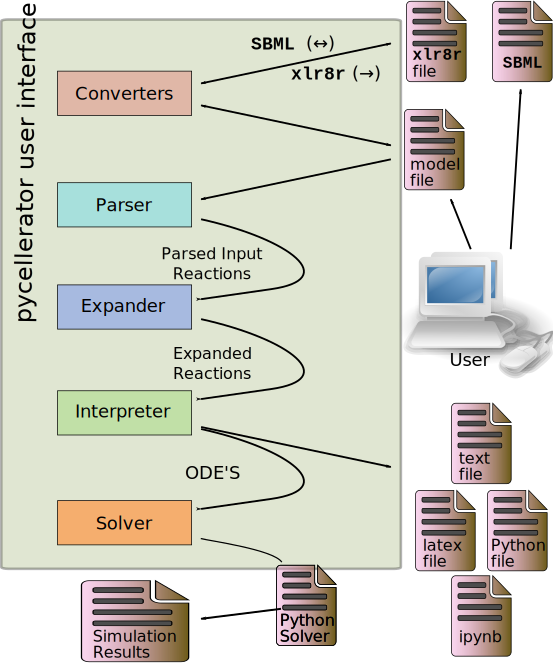
\includegraphics[width=.75\textwidth]{pyxlr8r-scheme.png}
\end{center}
\end{figure}




\chapter{Installation}

\section[Install Python]{Install a Basic Python System}

To use {\tt pycellerator}, python 2.7 and several python libraries must be installed on your computer. Python is free, open source, and available on all major operating systems.  This section provides an overview of how to install a basic python system on Windows, Macintosh OX, and Linux operating systems. 

\subsection{Installing on Windows}

There are two basic ways to install python: (1) install a ``commercial'' base distribution or (2) use a binary installer from  \url{https://www.python.org/downloads/windows/}{https://www.python.org/downloads/windows/}. There are several commercial distributions that provide free installers that will install the base python system for you. If you use a binary distribution, you will also have to install a number of other packages. The easiest commercial distributions to use are \textbf{Anaconda} and \textbf{Enthought Canopy}. 

\subsubsection{Anaconda Python}

To install Anaconda Python, go to \href{http://continuum.io/downloads}{http://continuum.io/downloads} and scroll down to select the appropriate installer for your operating system. This will download a file (e.g., Anaconda-2.3.0-x86\_64.exe, or something similar). 

Double click on the installer and follow the instructions to install python. 

After you are done, locate the {\tt Anaconda Command Prompt} from the windows search menu and type in the following. Type enter after line and wait until the command prompt (the name of the current folder)  is shown. 
\begin{lstlisting}
    conda update conda
    conda update ipython ipython-notebook ipython-qtconsole
    conda update numpy scipy sympy matplotlib
    python -m pip install --upgrade pip
    pip install pyparsing
    pip install pulp
\end{lstlisting}

\clearpage 

\subsubsection{Enthought Canopy}

As an alternative to Anaconda, Enthought Canopy is at \href{https://store.enthought.com/downloads/}{https://store.enthought.com/downloads/}. Pick your operating system from the button on the top of page and download the binary installer. 

After downloading the installation package (e.g., {\tt canopy-1.5.5-win-64.msi} or a similarly named file), double click on the installer to install python. It will be sufficient to answer all of the questions in the dialogs with the default values. 

When the installer is finished, the canopy dashboard should open automatically. You must run the dashboard at least once to finish the installation. The dashboard will open a menu that says ``Welcome to Canopy'' at the top. If the dashboard does not open, there should be a Canopy icon on your desktop. Click this to open the Canopy dashboard. If this icon is not installed, open Canopy from the windows search menu. If it does not appear, the installation has not completed properly.

From the Canopy dashboard select {\tt Edit > Preferences > General} and verify that Canopy is set as your default python environment. If it is not, click on the button that says ``Set as Default'', then click on ``OK.'' 

Then go to {\tt tools > package manager > available packages} and click on ``install all available packages.'

Then exit from Canopy by selecting {\tt File > Exit}. 

From the windows search menu, open {\tt Command Prompt} and type in the following commands, one at a time. Type enter after line and wait until the command prompt (the name of the current folder)  is shown. 

\begin{lstlisting}
    python -m pip install --upgrade pip
    pip install --upgrade numpy scipy sympy matplotlib
    pip install pyparsing
    pip install pulp
\end{lstlisting}

\subsubsection{Using the Binary Installers}

From \href{https://www.python.org/downloads/windows}{https://www.python.org/downloads/windows}, download the latest MSI installer for Python 2.7. At the time this was written, the file name was {\tt python-2.7.9.amd64.msi}. 

Locate the installer file, double click, and answer all the prompts. Make sure during the installation that python.exe and pip and checked off as visible to all. 

Next, download a Microsoft Visual C compiler for Python from \href{http://www.microsoft.com/en-us/download/details.aspx?id=44266}{http://www.microsoft.com/en-us /download/details.aspx?id=44266}. The installer file is called {\tt VCforPython27.msi}. Locate the installer, double click, and follow the instructions. Restart your computer after the installation is complete.

Open a command prompt (Windows search, type {\tt command prompt}) and enter the following:

\begin{lstlisting}
    python -m pip install --upgrade pip   
    pip install sympy pulp pyparsing setuptools
    pip install numpy scipy matplotlib
    pip install ipython[notebook]
\end{lstlisting}


\subsection{Installing on Macintosh OS}

If you have a Mac, then Python is already installed on your computer. The base system is pre-installed as part of the Mac operating system. The base system does not include the numerical libraries that are also required. You can either install these using {\tt pip} or install one of the commercial systems like Anaconda or Enthought Canopy. 

Follow the instructions for Windows if you want to install the commercial system. You will not need to install Visual C; instead, you may be prompted to download and install XCode tools from Apple during the installation process.  

\subsubsection{Upgrade Mac Python using \tt pip}

Locate the {\tt terminal} application in the {\tt utilities} folder and open it. Enter

\begin{lstlisting}
    sudo easy_install pip
\end{lstlisting}

When requested, enter you password (you must have administrator access on you Mac). If (when) you are prompted to install XCode from Apple, click yes, and follow the instructions on any dialog that follows. 

When the XCode installation is completed (or if it was not suggested), open a new terminal session and type in the following. Hit the enter key after each line and wait for the prompt (the name of the current working directory) before typing in the next line. 

\begin{lstlisting}
    pip install sympy pulp pyparsing
    pip install numpy scipy matplotlib
    pip install ipython[notebook]
\end{lstlisting}

If you have a virtual operating system like Parallels Desktop installed on your computer, make sure that Safari (or some other web browser such as Firefox or Chrome) is set as your default browser, and not Parallels. Otherwise ipython will try to open your virtual operating system every time it runs python. 


\subsection{Installing on Linux}

You can either install a base python system from your package manager, download binaries from \href{python.org}{python.org}, or build from source (also available at \href{python.org}{python.org}. Pycellerator requires python 2.7.X but is not compatible with python 3.x. 

The standard python installation includes its own package manage called {\tt pip}. If you install the base system from 
\href{python.org}{python.org} this should automatically be installed for your. Otherwise, you should look to also install {\tt pip} from your package manager. This allows you to bypass your package manager when updating python.

To upgrade to the latest version of {\tt pip},
\begin{lstlisting}
    python -m pip install --upgrade pip
\end{lstlisting}
To add any missing packages to python, 
\begin{lstlisting}
    pip install packagename
\end{lstlisting}
To upgrade to the latest version of any package,
\begin{lstlisting}
    pip install --upgrade package
\end{lstlisting}
Pycellerator needs the following packages which you can get from pip: {\tt pyparsing}, {\tt pulp}, {\tt sympy}, {\tt numpy}, {\tt scipy}, and{\tt matplotlib}.
\begin{lstlisting}
    pip install pyparsing
    pip install pulp
    pip install sympy
    pip install numpy
    pip install scipy
    pip install matplotlib
\end{lstlisting}
You can also put all the function names on a single line:
\begin{lstlisting}
    pip install pyparsing pulp sympy numpy scipy matplotlib
\end{lstlisting}
Binary installers and source code versions are also available for each of these packages. 

\begin{center}
\begin{tabular}{|ll|}
\hline
\textbf{Package} & \textbf{Project Home Page} \\ 
\hline
{\tt numpy} & \url{http://numpy.org/}\\
{\tt scipy} & \url{http://scipy.org/}\\
{\tt matplotlib}  & \url{http://matplotlib.sourceforge.net/}\\
{\tt pyparsing} & \url{http://pyparsing.wikispaces.com/} \\
{\tt sympy} &  \url{http://code.google.com/p/sympy/} \\
{\tt pulp} & \url{https://github.com/coin-or/pulp}\\

\hline
\end{tabular}
\end{center}


\section{Install libSBML}

If you want to work with SBML files, you will also need to install a version of libSBML that is appropriate for your operating system. Make sure to install a version that is compatible with Python. 

Follow the instructions at \href{http://sbml.org/Software/libSBML}{http://sbml.org/Software/libSBML} to find the appropriate binary installer for your operating system. 

You do not have to have libSBML installed if you do not plan on using SBML files. If libSBML is not installed, all non-SBML related functionality of pycellerator will be unaffected. 

The following describes how to install libSBML in ubuntu if you are primarily interested in using libSBML for python and not for other languages. It was taken from \url{http://sourceforge.net/projects/sbml/files/libsbml/5.11.6-experimental/binaries/Linux/} on 5 Sept 2015, and you should check for the latest information. 

\begin{enumerate}
\item Install the  prerequisite software packages installed on your operating system: \CODE{python-dev}, \CODE{libxml2-dev}, \CODE{libz-dev}, and \CODE{libbz2-dev}.
\begin{lstlisting}
  sudo apt-get install python-dev libxml2-dev libz-dev libbz2-dev
\end{lstlisting}
\item From the terminal type:
\begin{lstlisting}
  sudo pip install python-libsbml
\end{lstlisting}
\end{enumerate}

For windows, the latest (as of 5 Sept 2015) binary python installers are at \url{http://sourceforge.net/projects/sbml/files/libsbml/5.11.4/stable/Windows/64-bit/python/}. These installers will only install libSBML for python, and not for other languages. 

The Mac installers are at \url{http://sourceforge.net/projects/sbml/files/libsbml/5.11.4/stable/Mac\%20OS\%20X/} and the instructions given for installation are similar to those for linux.

\section{Install pycellerator}

The procedure to install pycellerator follows. 

  

\begin{enumerate}
\item Get the latest \textbf{release} from github. This can be found at \url{https://github.com/biomathman/pycellerator/releases}. Download the file \CODE{Install-pycellerator-v-X.zip}, where \CODE{X} is the latest version number. This will be a compressed archive (zip file) of the files you need to install pycellerator.

\item  Unzip the archive.  Copy the folder \CODE{pycellerator} (e.g., drag and drop the entire folder) to wherever you want to keep your pycellerator files. For example, this may be a folder in your home directory. If your home folder is \CODE{johnsmith}, and you drag \CODE{pycellerator} onto your home folder, then your \CODE{pycellerator} folder will be \CODE{johnsmith/pycellerator}, i.e., the folder \CODE{pycellerator} inside your home folder. 

\item Inside the \CODE{pycellerator} folder is detailed documentation in the 
file \CODE{pycellerator.pdf} (the file you are reading now). Chapter 2 gives detailed instructions on how to
install Python (if you don't already have it installed); and what additional
Python libraries are needed and how to get them.

\item A quickstart check of the command line utility, from inside the \CODE{pycellerator} folder, type the following into the terminal:
\begin{lstlisting}
    python pycellerator.py solve -in Gold1.model -plot
\end{lstlisting}

\item For a quickstart check of the ipython notebook, type the following into the terminal:
\begin{lstlisting}
    ipython notebook
\end{lstlisting}
Navigate to the notebook \CODE{demo.ipynb} and open it.

\end{enumerate}




\chapter[Arrows]{pycellerator Arrow Reference}
\label{chapter:arrows}

\section{Introduction}

Reactions in pycellerator are specified in textfiles using a arrow based language that can be typed using any standard ASCII or UTF keyboard. All of the characters needed to type a reaction exist on standard US keyboards. A summary of the arrow forms available in pycellerator is given in Table 3.1. 

The canonical form for an arrow form  is 
\begin{equation*}
{\text{\tt[LHS {\rm{\it arrow}} RHS, mod[{\rm {\it modifiers}}], rates[{\rm {\it rate constants}}]]}}
\end{equation*}
or
\begin{equation*}
{\text{\tt[LHS {\rm{\it arrow}} RHS, rates[{\rm {\it rate constants}}]]}}
\end{equation*}
All of the square brackets are required and:

{\tt LHS} indicates a species, list of species, or sum of species that give the input to the reaction. Depending on the type of reaction, their concentrations or amounts may or may not change as a result of the reaction, but they will always affect the calculation of the output species. 

{\tt RHS} indicates a species, list of species, or sum of species that give the output of the reaction. Each species in {\tt RHS} will will normally change in concentration or amount as a result of the reaction. 

{\it arrow} determines the type of reaction. It typically looks something like ${\text {\tt ->, -->, =>, |->}}$, etc. 

{\it modifiers} indicates a list of species that affect the output of the reaction; like input reaction, their concentrations may or may not be affected by the reactions. The definition of whether a species goes in the {\tt mod} or {\it modifiers} list depends on the definition of the reaction in the following sections, and not on the biochemical process. This is a computational distinction only. In general, {\tt modifiers} correspond to catalysts in enzymatic reactions. The normal distinction used is that for \textbf{catalytic} arrows  (e.g., ${\text {\tt |->}}$) the amount of catalyst does not change, but in \textbf{enzymatic} arrows  (e.g., ${\text {\tt =>, <=>}}$) the amount of enzyme may, in fact, change. 


\pagebreak


\renewcommand{\arraystretch}{2.5}
%\begin{table}[ht]%\caption{toodly doo}
\begin{scriptsize}
\begin{center}
Table 3.1
\end{center}
\begin{tabular}{|p{1in}|lp{3in}|p{1.5in}|l|}
\hline\textbf{Name} &\multicolumn{2}{|l|}{\textbf{Arrow}} & \textbf{Typical ODE Term}&\textbf{Ref} \\
\hline
\LJ{Simple Mass Action}&1& {\tt [X $->$ Y, k]}&\multirow{2}{*}{$\displaystyle{(s_{i,r}-s_{i,l}) k \prod_{i\in \text{LHS}}\text{X}_i^{e_i}}$}&\ref{section:Simple-Mass-Action}\\
\cline{2-3}\cline{5-5}\LJ{Mass Action, Stoichiometry}&2& {\tt [e1 X1 + e2 X2 + $\cdots$ $->$ s1 Y1 + s2 Y2 + $\cdots$, k]} & & \ref{section:simple-mass-action-stoich}\\
\cline{2-5}\LJ{Mass Action, Reversible}&3& {\tt [e1 X1 + $\cdots$ $<->$ s1 Y1 + $\cdots$, rates[k1,k2]]} &  Expanded into a pair of type (1) or (2) reactions.&\ref{section:reversible-mass-action}\\
\cline{2-5}\LJ{Simple Catalytic}&4&
\LMM{
$\text{\tt [e1 A1 + e2 A2 + }\cdots  $
$\text{\tt --> s1 B1 + s2 B2 +} \cdots \text{\tt ,} $ 
$\text{\tt mod[X], k]}$} & Expanded into a single  type (1) or (2) reaction. &\ref{section:simple-mass-action-cat}\\
\cline{2-5}\LJ{Catalytic, w/ Intermediate Complex}&5& {\tt [A => B, mod[X], rates[k1, k2, k3, k4]]} & Expanded into three or four type (1) reactions &\ref{section:cat-mass-action}\\
\cline{2-5}\LJ{Catalytic, Reversible, w/ Int. Complex}&6&{\tt [A <=> B, mod[X,Y], rates[k1, k2,...,k8]]} & Expanded into two type (5) reactions. & \ref{section:cat-mass-action-reversible}\\
\cline{2-5}\LJ{Catalytic, Two Int. Species}&7&{\tt [A :=> B, mod[E], rates[k1,k2,...,k6]} & Expanded into six type (1) reactions & \ref{section:cat-mass-action-two-complex}\\
\hline\multirow{2}{*}{\textbf{Hill Functions}}&8&{\tt [A |-> B, Hill[v,n,K,$\alpha$,T]]}&\multirow{2}{*}{$\displaystyle{\dfrac{vEk(\sum T_i A_i + \alpha)^n}{K^n + (\sum T_i A_i + \alpha)^n}}$}&\multirow{2}{*}{\ref{section:Hill}}\\
\cline{2-3}&9&{\tt [A |--> B, mod[E], Hill[v,n,K,$\alpha$,T]]}&&\\
\hline{\multirow{2}{*}{\LJ{GRN (Genetic Regulatory Network Model)}}}      &10&{\tt [A |-> B, GRN[v,$\beta$,n,h]]}& \multirow{2}{*}{$\displaystyle{\dfrac{vE}{1+\exp(-h-\sum\beta_i A_i^{n_i})}}$}&\multirow{2}{*}{\ref{section:GRN}}\\
\cline{2-3}&11&{\tt [A |--> B, mod[E], GRN[v,$\beta$,n,h]]}&&\\
\hline{\multirow{2}{*}{\textbf{S-System}}}      &12&{\tt [A |-> B, SSystem[$\tau$, k$_{+}$, k$_{-}$, c$_{+}$,c$_{-}$]]}& \multirow{2}{*}{$\dfrac{k_+ \prod A_i^{C_{i,+}} -k_{-}\prod A_{i}^{C_{i,-}}}{\tau}$}&\multirow{2}{*}{\ref{section:SSystem}}\\
\cline{2-3}&13&{\tt [A |--> B, mod[E], SSystem[$\tau$, k$_{+}$, k$_{-}$, c$_{+}$,c$_{-}$]]}&&\\
\hline\multirow{2}{*}{\LJ{MMH (Michaelis- Menten- Henri)}}& 14 &{\tt[A :->B, MMH[K,v]]} or  {\tt[A :->B, MMH[k1,k2,k3]]} &
\multirow{2}{*}{$\dfrac{vAE}{K+A}$ or $\dfrac{k_3 A E}{(k_2+k_3)/k_1 + A}$}& \multirow{2}{*}{\ref{subsection:MMH}} \\
\cline{2-3} & 15 &{\tt[A :-->B, mod[X], MMH[K,v]]} or  {\tt[A :->B,mod[X], MMH[k1,k2,k3]]} &&  \\
\hline
\LJ{Rational Function} & 16 & {\tt[[[A1,A2,..],[X1,X2,..]]==>S,rational[a,d,m,n]]}&$\dfrac{a_0 + \sum a_i A_i^{n_i}}{d_0 + \sum d_i X_i^{m_i}} $ & \ref{subsection:Rational} \\
\hline\multirow{2}{*}{\LJ{MWC (Monod-Wyman-Changeaux)}}&17&
{\tt[S==>P, mod[E], MWC[k, n, c, L, K]]} & 
\multicolumn{2}{l|}{

$\dfrac{k \mathcal{E} \left(c L
   s (c s+1)^{n-1}+s
   (s+1)^{n-1}\right)}{L (c
   s+1)^n+(s+1)^n}$ }
\\
\cline{2-3}\cline{5-5} &18& {\tt[S==>P, mod[E, [[A1,A2,..],[I1,I2,..]], MWC[k, n, c, L, K]]}&See reference for multiple Activator/Inhibitor equations.&\ref{subsection:MWC}\\
\hline \LJ{NHCA (Non-hierarchical coop. act.}&19&{\tt A|-> B, NCHA[v, Tp, Tm, n, m, k]}& 
\LM{$\dfrac{vA^m}{kB^m+A^m}$,   $A\hspace{-2pt}=\hspace{-2pt}1\hspace{-2pt}+\hspace{-2pt}T_{p}X^n$, $B\hspace{-2pt}=\hspace{-2pt}1\hspace{-2pt}+\hspace{-2pt}T_{m}X^n$} & \ref{section:NHCA}\\
\hline
\end{tabular}


\newpage

\begin{center}
Table 3.1 (continued)
\end{center}
\begin{tabular}{|p{1in}|lp{3in}|p{1.5in}|l|}
\hline\textbf{Name} &\multicolumn{2}{|l|}{\textbf{Arrow}} & \textbf{Typical ODE Term}&\textbf{Ref} \\

\hline 
\multirow{2}{*}{\LJ{USER}} &20&  $\TT{[ X1+X2+}\cdots \TT{|->Y, USER[v, T, n, h, f]]}$ & $v f(h-\sum T_i P_i^{X_i})$&\ref{subsection:USER} \\
&& {\tt f} should by a Python lambda expression of a single variable && \\
\hline
\multirow{2}{*}{\LJ{using}}&21& $\TT{[s1*X1+s2*X2+} \cdots {\tt -> q1*X1+}\cdots\tt{, using["expr"]]}$ & $X_i' = q_i-s_i)X_i$ & \ref{section:USERST}\\
&& {\tt expr} should be Python infix expression depending on variables defined in the model. &&
\\
\hline
\end{tabular}

\vspace{24pt}


\end{scriptsize}
%\end{table}




\renewcommand{\arraystretch}{1.0}



{\tt rates} is a keyword that varies with the type of arrow; typical keywords include {\tt MWC} (for Monod-Wyman-Changeaux); {\tt MMH} (for  Michaelis-Menten-Henri); {\tt Hill} (for Hill functions); and so forth. 

{\it rate constants} is a list of symbols or numbers that give the rate constants or other parameters used in the reaction equation. The definition of these parameters is different for each type of reaction, and is described in the following sections and subsections. 

%************************************************************************
\section[Equations for Rates]{Substituting Equations for Rate Constants}
\label{section:EARC}

In any of the arrow expressions that follow in the remainder of the chapter, any rate constant may be replaced by any valid Python expression in quotation marks. Fore example, the hypothetical reaction

\begin{verbatim}
    [X -> Y, "v/(K+X)"]
\end{verbatim}

is perfectly valid. Since the reaction itself is written in the form of a mass action equation, the expression is treated as a rate constant $k$ and the odes are $\TT{[Y]}'==\TT{[X]}'=k\TT{[X]}$, where $k$ is to be replaced with the expression in quotes. It will thus produce the differential equation terms:
\begin{align*}
\TT{[Y]}' = -\TT{[X]}' = \dfrac{v \TT{[X]}}{K+\TT{[X]}}
\end{align*}

This allows users to define virtually any rate law in a reaction. 

See also User Defined Regulatory Arrows in section \ref{subsection:USER} and User Defined Stoichiometric Arrows in section \ref{section:USERST}. User defined stoichiometric arrows will not multiply the expression by the mass-action product (the product of the species on the left, each raised to their individual stoichiometries), as this method will, but will retain a balance of stoichiometry, with the each reactant and product changing unless their stoichiometries are balanced. The user defined regulatory reactions, on the other hand, will  not generate any ODE terms for the reactants on the left-hand side of the arrow. 

%************************************************************************
\section{Indexed Species}

An array index may be attached to a species variable using parenthesis as a delimiter, as in the following example:


{\tt \hspace{.5in} [K(3,0) <=> K(3,1), mod[RAFK, RAFph], rates[a1,d1,k1,0,a2,d2,k2,0]]}

The index may also be applied to a modifier variable, and within the initial condition section of the model file, e.g., 

{\tt \hspace{.5in} K[3,0] = 0.7 }

See the examples chapter (MAPK cascade with indexed stages) for an example. 

\paragraph{Implementation Note:} When instantiated in the {\tt Reaction} class, the indices are expanded into the variable name, and separated with underscores e.g., {\tt K[i,j]} becomes {\tt K\_i\_j}; this variables are implemented in this expanded form in the solver and displayed this way on plots. 


%************************************************************************
\section[{\tt Nil} \& {\tt EmpytSet} Species] {The {\tt Nil} and {\tt EmptySet} Species}

The species {\tt Nil} is used to represent the vacuum or the empty set. No ODE term is ever generated for the species {\tt Nil}. 

The variable {\tt EmptySet} is predefined in Sympy and should not be used in models. If it is used in an SBML file it will be converted to {\tt Nil}. 


For example, the reaction
$$\TT{[Nil->A, k]}$$
denotes creation and represents a special case of mass-action reaction, in which $A'=k$ (rather than $A'=k\times\tt{[Nil]}$ as it would be in any other reaction). 

Similarly, the reaction
$$\TT{[A->Nil, k]}$$
represents destruction, and is treated normally for the species {\tt A}, but no differential equation term is generated for {\tt Nil}.
%************************************************************************
\section{Mass Action Arrows}

\subsection{Simple Mass Action}
\label{section:Simple-Mass-Action}

\underline{{\tt pycellerator} Arrow}: \begin{center}
\fbox{{\tt [X $->$ Y, k]}}
\end{center}

{\tt X, Y} are identifiers representing chemical species;  {\tt k} is either an identifier or a number representing a rate constant. 

\underline{Equivalent {\tt xlr8r} Arrow}: \begin{center}
{\tt \{X $\to$ Y, k\}}
\end{center}

\underline{Typical biochemical notation}: $$\text{X} \overset{k}{\to} \text{Y}$$

\underline{Interpreted differential equation terms}: 
\begin{align*}
\dfrac{d\text{Y}}{dt} = 
-\dfrac{d\text{X}}{dt} = k \text{X}
\end{align*}



\subsection{Simple Mass Action, with stoichiometry}
\label{section:simple-mass-action-stoich}


\underline{{\tt pycellerator} Arrows}: \begin{center}
\fbox{{\tt [e1 X1 + e2 X2 + $\cdots ->$ s1 Y1 + s2 Y2 + $\cdots$ , k]}},

\fbox{{\tt [e1 $*$ X1 + e2 $*$ X2 + $\cdots ->$ s1 $*$ Y1 + s2 $*$ Y2 + $\cdots$ , k]}}
\end{center} 

\underline{Species}: {\tt X1, X2, ...,  Y1,Y2, ...} are identifiers representing chemical species.

\underline{Stoichiometry}: {\tt e1, e2, ..., s1, s2, ...} are either identifiers or numbers representing stoichiometries before and after the reaction. The multiplication symbols ($*$) are optional. 

If any stoichiometry is an identifier, there must be either an $*$ or a blank space between it and the corresponding species identifier. If the stoichiometry is numerical the blank space is optional. For example {\tt 3X}, {\tt 3$*$X}, and {\tt 3\ X}, will all be treated as a species {\tt X} with stoichiometry 3, and  {\tt s H20} and {\tt s$*$H20} will both be interpreted as a species {\tt H20} with stoichiometry {\tt s}, whereas {\tt sH20} will be interpreted as a single species {\tt sH20} with a stoichiometry of 1. 


\underline{Equivalent {\tt xlr8r} Arrow}: \begin{center}
{\tt \{e1 X1 + e2 X2 + $\cdots$  $\to$ s1 Y1 + s2 Y2 + $\cdots$, k\}}
\end{center}

\underline{Typical biochemical notation}: $$e_1 \text{X}_1 + e_2 \text{X}_2 + \cdots \overset{k}{\to} s_1\text{Y}_1 + s_2\text{Y}_2 + \cdots$$

\underline{Interpreted differential equation terms}: 
\begin{align*}
\dfrac{d\text{U}_i}{dt} &=
(s_{i,r}-s_{i,l}) k \text{X}_1^{e_1} \text{X}_2^{e_2} \cdots
\end{align*}
where $s_{i,r}$ and $s_{i,l}$ are the stoichiometry of $\text{U}_i$ on the right-hand-side and left-hand-side of the reaction, respectively, and $\text{U}_i$ refers to any species either on either side of the equation (either an $\text{X}_i$ or a $\text{Y}_i$). The product is taken over all the terms on the left-hand-side of the reaction, each term raised to its respective stoichiometry (this is also known as the law of mass action).  


\subsection{Simple Mass Action, Catalyzed}
\label{section:simple-mass-action-cat}

\underline{{\tt pycellerator} Arrows}: \begin{center}
\fbox{{\tt [e1 A1 + e2 A2 + $\cdots -->$ s1 B1 + s2 B2 + $\cdots$, mod[X], k]}},

\fbox{{\tt [e1 $*$ A1 + e2 $*$ A2 + $\cdots -->$ s1 $*$ B1 + s2 $*$ B2 + $\cdots$, mod[X], k]}}
\end{center} 
The stoichiometries are optional. Multiplication symbols ($*$) or spaces are optional if numerical stoichiometries are used, but are required if symbolic stoichiometries are used. 

\underline{Equivalent {\tt xlr8r} Arrow}: 
$$\tt\{e_1 A_1 + e_2 A_2 + \cdots \overset{X}{\to} s_1 B_1 + s_2 B_2 + \cdots, k\}$$

\underline{Typical biochemical notation}: $$\tt{X + e_1 A_1 + e_2 A_2 + \cdots \overset{k}{\to} S + s_1 B_1 + s_2 B_2 + \cdots}$$

\underline{Interpreted differential equation terms}: 
The reaction is expanded into a single reaction of the form 

 \begin{center}
{\tt [X + e1 A1 + e2 A2 + $\cdots ->$ X + s1 B1 + s2 B2 + $\cdots$, mod[X], k]}
\end{center} 
as described in section \ref{section:simple-mass-action-stoich}.


\subsection{Reversible Mass Action}
\label{section:reversible-mass-action}


\underline{{\tt pycellerator} Arrow}: \begin{center}
\fbox{{\tt [e1 X1 + e2 X2 + $\cdots <->$ s1 Y1 + s2 Y2 + $\cdots$ , rates[k1,k2]]}} 
\end{center}
The stoichiometries are optional.

\underline{Equivalent {\tt xlr8r} Arrow}: \begin{center}
{\tt \{e1 X1 + e2 X2 + $\cdots$  $\rightleftarrows$ s1 Y1 + s2 Y2 + $\cdots$, k1, k2\}}
\end{center}
\underline{Typical biochemical notation}: $$e_1 \text{X}_1 + e_2 \text{X}_2 + \cdots \underset{k2}{\overset{k}{\rightleftarrows}} s_1\text{Y}_1 + s_2\text{Y}_2 + \cdots$$



\underline{Interpreted differential equation terms}: 

This arrow is reduced to the pair of simple mass action equations, as described in section \ref{section:simple-mass-action-stoich}: 

\begin{center}
{\tt [e1 X1 + e2 X2 + $\cdots ->$ s1 Y1 + s2 Y2 + $\cdots$ , k1]}\\
{\tt [s1 Y1 + s2 Y2 + $\cdots ->$ e1 X1 + e2 X2 + $\cdots$  , k2]}
\end{center}

The contributions to the differential equations are then computed as described in section \ref{section:simple-mass-action-stoich}.

\subsection{Catalytic Mass Action, Intermediate Substrate/Catalyst Complex Formation}
\label{section:cat-mass-action}

\underline{{\tt pycellerator} Arrow}: \begin{center}
\fbox{\tt 
[A => B, mod[X], rates[k1, k2, k3, k4]]
} 
\end{center}
\underline{Equivalent {\tt xlr8r} Arrow}:
$$\tt\{A \overset{X}{\rightleftarrows} B,k1,k2,k3,k4 \}$$

\underline{Typical biochemical notation}: 
$$ X+A\underset{k_2}{\overset{k_1}  \rightleftarrows } XA \underset{k_4}{ \overset{k_3}{\rightleftarrows}} X+B$$

Typically {\tt k4} is omitted, in which case it is assumed to be zero. If fewer than four parameters are given they are zero-filled to the right. 

This arrow is expanded into the following collection of simple mass action arrows as described in section \ref{section:simple-mass-action-stoich}:

\begin{center}
{\tt [X + A -> A\_X, k1]}\\
{\tt [A\_X -> X + A, k2]}\\
{\tt [A\_X -> X + B, k3]}\\
{\tt [X + B -> B\_X, k4]}
\end{center}

The name of the intermediate complex is automatically generated by concatenating the names of the substrate and the catalyst with an underscore. The resulting contributions to the differential equations for {\tt [A], [B], [X]} and {\tt [X\_A]} in the above scheme are then: 

\begin{align*}
{\tt [A]}'&=k_2 {\tt [A\_X]} - k_1 {\tt [A][X]}\\
{\tt [B]}'&=k_3 {\tt [A\_X]} -  k_4 {\tt [B][X]}\\
{\tt [X]}'&=-k_1 {\tt [A][X]} + (k_2+k_3) {\tt [A\_X]}- k_4 {\tt [B][X]}\\
{\tt [A\_X]}'&= k_1 {\tt [A][X]} - (k_2 + k_3) {\tt [A\_X]} + k_4 {\tt [B][X]}
\end{align*}

\subsection{Catalytic Mass Action, Intermediate Substrate/Catalyst Complex Formation, Reversible}
\label{section:cat-mass-action-reversible}
\underline{{\tt pycellerator} Arrow}: \begin{center}
\fbox{\tt 
[A <=> B, mod[X, Y], rates[k1, k2, k3, k4, k5, k6, k7, k8]]
} 
\end{center}

If fewer than 8 rate constants are given they are zero-filled to the right. 

\underline{Equivalent {\tt xlr8r} Arrow}:
$$\tt\{A \underset{Y}{\overset{X}{\rightleftarrows}} B,k1,k2,k3,k4, k5, k6, k7, k8 \}$$

\underline{Typical biochemical notation}: 
$$ X+A\underset{k_2}{\overset{k_1}  \rightleftarrows } XA \underset{k_4}{ \overset{k_3}{\rightleftarrows}} X+B$$
$$ Y+B\underset{k_6}{\overset{k_5}  \rightleftarrows }  YB \underset{k_8}{ \overset{k_7}{\rightleftarrows}} Y+A$$

When computing the differential equation contribution, this arrow is expanded into the following pair of catalytic mass action reactions with intermediate complex formation, as described in section \ref{section:cat-mass-action}: 
\begin{center}
{\tt [A => B, mod[X], rates[k1, k2, k3, k4]]}\\
{\tt [B => A, mod[Y], rates[k5, k6, k7, k8]]}
\end{center}
These reactions are subsequently broken down in simple mass action reactions as described in section \ref{section:simple-mass-action-stoich}. 
\begin{center}
{\tt [A+X->A\_X,k1]}\\
{\tt [A\_X->A+X,k2]}\\
{\tt [A\_X->B+X,k3]}\\
{\tt [B+X->A\_X,k4]}\\
{\tt [B+Y->B\_Y,k5]}\\
{\tt [B\_Y->B+Y,k6]}\\
{\tt [B\_Y->A+Y,k7]}\\
{\tt [A+Y->B\_Y,k8]}
\end{center}
The contributions to the ODE are computed as described based on these reduced reactions, as described in \ref{section:simple-mass-action-stoich}: 
\begin{align*}
{\tt [A]}'    &=  k_2{\tt [A\_X]} + k_7{\tt [B\_Y]} - A*X*k1 - A*Y*k8\\
{\tt [B]}'    &=  k_3{\tt [A\_X]} + k_6{\tt [B\_Y]} - B*X*k4 - B*Y*k5\\
{\tt [A\_X]}' &= -(k_2+k_3){\tt [A\_X]} + k_1{\tt [A][X]} + k_4{\tt [B][X]}\\
{\tt [B\_Y]}' &= -(k_6+k_7){\tt [B\_Y]} + k_8{\tt [A][Y]} + k_5{\tt [B][Y]}\\
{\tt [Y]}'    &=  (k_6+k_7){\tt [B\_Y]} - k_8{\tt [A][Y]} - k_5{\tt [B][Y]}\\
{\tt [X]}   ' &=  (k_2+k_3){\tt [A\_X]} - k_8{\tt [A][X]} - k_4{\tt [B][X]}
\end{align*}


\subsection{Catalytic Mass Action with Substrate/Enzyme and Product/Enzyme Intermediate Complexes}
\label{section:cat-mass-action-two-complex}
\underline{{\tt pycellerator} Arrow}: \begin{center}
\fbox{\tt 
[A :=> B, mod[X], rates[k1, k2, k3, k4, k5, k6]]
} 
\end{center}

\underline{Equivalent {\tt xlr8r} Arrow}:
$$\tt\{A \overset{X}{\rightleftharpoons} B,k1,k2,\dots,k6 \}$$

\underline{Typical biochemical notation}:
$$ A+X\underset{k_2}{\overset{k_1}  \rightleftarrows } AX \underset{k_4}{ \overset{k_3}{\rightleftarrows} } BX \underset{k_6}{\overset{k_5}{\rightleftarrows}} B+X$$


\underline{Interpreted differential equation terms}:
This arrow is expanded into the following collection of simple mass action arrows as described in section \ref{section:simple-mass-action-stoich}:
\begin{center}
{\tt [A+X->A\_X,k1]}\\
{\tt [A\_X->A+X,k2]}\\
{\tt [A\_X->B\_X,k3]}\\
{\tt [B\_X->A\_X\,k4]}\\
{\tt [B\_X->B+X,k5]}\\
{\tt [B+X->B\_X,k6]}
\end{center}
These are then converted into terms in the differential equations as described above in \ref{section:simple-mass-action-stoich}:
\begin{align*}
{\tt [A]'}    &= k_2{\tt [A\_X]} - k_1 {\tt [A][X]}\\
{\tt [X]'}    &= k_2{\tt [A\_X]} + k_5 {\tt [B\_X]} - k_1 {\tt [A][X]} - k_6 {\tt [B][X]}\\
{\tt [B]'}    &= k_5{\tt [B\_X]} - k_6 {\tt [B][X]}\\
{\tt [B\_X]'} &= k_3{\tt [A\_X]} - (k_4+k_5) {\tt [B\_X]} + k_6 {\tt [B][X]}\\
{\tt [A\_X]'} &= k_4{\tt [B\_X]} - (k_2+k3_) {\tt [A\_X]} + k_1 {\tt [A][X]}
\end{align*}



\section{Equilibrium / Steady-State Models}
\subsection{Michaelis-Menten-Henri (MMH) Reactions }
\label{subsection:MMH}
\underline{{\tt pycellerator} Arrows}:
%\begin{center}
%\begin{minipage}{3in}
\begin{align}
&\boxed{\text {\tt [A :-> B, MMH[K, v]]}}\label{eq:MM1}\\
&\boxed{\text {\tt [A :-> B, MMH[k1, k2, k3]]}}\label{eq:MM2}\\
&\boxed{\text {\tt [A :-> B, mod[X], MMH[K, v]]}} \label{eq:MM3}\\
&\boxed{\text {\tt [A :-> B, mod[X], MMH[k1, k2, k3]]}}\label{eq:MM4}
\end{align}
%\end{minipage}
%\end{center}

\underline{Equivalent {\tt xlr8r} Arrow}: 
\begin{align*}
\{ {\tt A} &\implies {\tt B, MM[K,v]}\} \\
\{ {\tt A} &\implies {\tt B, MM[k1, k2, k3]}\} \\
\{ {\tt A} &\overset{\tt X}{\implies} {\tt B, MM[K,v]}\}\\
\{ {\tt A} &\overset{\tt X}{\implies} {\tt B, MM[k1, k2, k3]}\}
\end{align*}


\underline{Typical Biochemical Notation}: 

Non-standard. 

\underline{Interpreted Differential Equation}:

\begin{align*}
{\tt[B]'} &= -{\tt[A]'} = \dfrac{v{\tt[A]}}{K+{\tt[A]}} &\text{for \ref{eq:MM1}}\\
{\tt[B]'} &= -{\tt[A]'} = \dfrac{k_3 {\tt[A]}}{(k_2+k_3)/k_1+{\tt[A]}} &\text{for \ref{eq:MM2}}\\
{\tt[B]'} &= -{\tt[A]'} = \dfrac{v{\tt[A][X]}}{K+{\tt[A]}} &\text{for \ref{eq:MM3}}\\
{\tt[B]'} &= -{\tt[A]'} = \dfrac{k_3{\tt[A][X]}}{(k_2+k_3)/k_1+{\tt[A]}} &\text{for \ref{eq:MM4}}
\end{align*}

\subsection{Monod-Wyman-Changeaux (MWC) Reactions}
\label{subsection:MWC}
\underline{{\tt pycellerator} Arrows}:
\begin{align}
&\boxed{\text{\tt[S==>P,mod[E],MWC[k,n,c,L,K]]}} \label{eq:MWC1}\\
&\boxed{\text{\tt[[S1,S2,..]==>P,mod[E,[A1,A2,..],[I1,I2,..]],MWC[k,n,c,L,},K_1\text{\tt]]}} \label{eq:MWC2}\\\
&\text{where }K_1 = \TT{[K}_{\TT{S1}}\TT{,K}_{\TT{S2}}\TT{,..],[K}_{\TT{A1}}\TT{,K}_{\TT{A2}}\TT{,..],[K}_{\TT{I1}}\TT{,K}_{\TT{I2}}\TT{,..]}\\
&\boxed{
\text{\tt[[S1,S2,..]==>P},\text{\tt mod[E,[A1,A1,..],[I1,I2,..],}X \text{\tt],} \text{\tt MWC[k,n,c,L,}K_2\text{\tt]]}
} \label{eq:MWC3}\\
&\text{where }
X = \overbrace{\TT{[CS}_{11}\TT{,CS}_{12}\TT{,..]}}^{\text{{\tt S1} inhibitors}} \TT{,}
    \overbrace{\TT{[CS}_{21}\TT{,CS}_{22}\TT{,..]}}^{\text{{\tt S2} inhibitors}} \TT{,..,}\nonumber\\&\hspace{1in}
    \underbrace{\TT{[CA}_{11}\TT{,CA}_{12}\TT{,..]}}_{\text{{\tt A1} inhibitors}} \TT{,}
    \underbrace{\TT{[CA}_{21}\TT{,CA}_{22}\TT{,..]}}_{\text{{\tt A2} inhibitors}}  \TT{,..}\\&\hspace{1in}
\text{are competitive inhibitors, and, } \nonumber\\
&\text{where }K_2 = \TT{[K}_{\TT{S1}}\TT{,K}_{\TT{S2}}\TT{,..],[K}_{\TT{A1}}\TT{,K}_{\TT{A2}}\TT{,..],[K}_{\TT{I1}}\TT{,K}_{\TT{I2}}\TT{,..],..}\nonumber\\
&\hspace{1in}\TT{[K}_{\TT{CS11}} \TT{,K}_{\TT{CS12}}\TT{,..],[K}_{\TT{CS21}}\TT{, K}_{\TT{CS22}}\TT{,..]..}\nonumber \\
&\hspace{1in}\TT{[K}_{\TT{CA11}}\TT{,K}_{\TT{CA12}}\TT{,..],[K}_{\TT{CA21}}\TT{,K}_{\TT{CA22}}\TT{,..],..}
\end{align}

\underline{Equivalent {\tt xlr8r} Arrow}: 
\begin{align*}
&\TT{\{S} \overset{\TT{Enz}}{\implies} \TT{P, MWC[k,n,c,L,K]} \TT{\}}&\text{(for \eqref{eq:MWC1})}\\
&\TT{\{} \underset{\text{\tt \{\{A1,A2,..,\},\{I1,I2,..\}\} }}{ {\TT{S} \overset{\TT{Enz}}{\implies} \TT{P}}} \TT{, MWC[k,n,c,L,K,..]} \TT{\}}&\text{(for \eqref{eq:MWC2})}\\
&\TT{\{} \underset{\text{\tt \{\{A1,A2,..,\},\{I1,I2,..\},\{CS1,..\},..,\{CA1,..\},..\} }}{ {\TT{S} \overset{\TT{Enz}}{\implies} \TT{P}}} \TT{, MWC[k,n,c,L,K,..]} \TT{\}}&\text{(for \eqref{eq:MWC3})}
\end{align*}

\underline{Typical Biochemical Notation}: 

Not standardized. 

\underline{Interpreted Differential Equation}:

The ODE terms for equation \eqref{eq:MWC1} are based on the theory of \cite{MWC}. Let $c=\TT{[S]/K}$. Then 

\begin{align*}
\TT{[P]}' = -\TT{[S]}' &= \TT{[E]}\dfrac{{s \left(1 + s\right)^{n-1}} + {L s c \left(1 + s c\right)^{n-1}}}
              {\left(1 + s\right)^{n} + L \left(1 + {s c}\right)^{n-1}}
              &\text{ for \eqref{eq:MWC1}}
\end{align*}
The terms for reactions \eqref{eq:MWC2} and \eqref{eq:MWC3} are described in \cite{GMWC}. For the first arrow, let 
\begin{align*}
s_j = \dfrac{\TT{[S]}_j}{\TT{K}_{\TT{S}j}}, 
a_j = \dfrac{\TT{[A]}_j}{\TT{K}_{\TT{a}j}}, 
i_j = \dfrac{\TT{[I]}_j}{\TT{K}_{\TT{I}j}}
\end{align*}
Then
\begin{align*}
\TT{[P]}' = -\TT{[S]}' &= \TT{[E]}\dfrac{
{\prod(1+a_j)^n \prod s_j \prod(1 + s_j)^{n-1}} + {L \prod(1+i_j)^n \prod (cs_j ) \prod (1 + c s_j)^{n-1}}}
              {\prod(1+a_j)^n\prod (1 + s_j)^{n} + L \prod(1+i_j)^n\prod(1 + {c s_j})^{n-1}}
              &\text{ for \eqref{eq:MWC2}}
\end{align*}
For \eqref{eq:MWC3} we can also normalize the competitive inhibitors as
\begin{align*}
&\overline{s_j} = c \sum_k \dfrac{\TT{[CS]}_{jk}}{\TT{K}_{\TT{CS}jk}},\hspace{.5in}
\overline{a_j} = c \sum_k \dfrac{\TT{[CA]}_{jk}}{\TT{K}_{\TT{CA}jk}}\\
\end{align*}
and then
\begin{align*}
\TT{[P]}' &= -\TT{[S]}' \\
&= \TT{[E]}\dfrac{
{\prod(1+a_j\overline{a_j})^n \prod s_j \prod(1 + s_j+\overline{s_j})^{n-1}} + {L \prod(1+i_j)^n \prod (cs_j ) \prod (1 + c s_j + \overline{sj})^{n-1}}}
              {\prod(1+a_j+\overline{a_j})^n\prod (1 + s_j)^{n} + L \prod(1+i_j)^n\prod(1 + {c s_j} + \overline{s_j})^{n-1}}
              &\text{ for \eqref{eq:MWC3}}
\end{align*}

 
\subsection{Non-regulatory Hill Functions}
These are described below in section \ref{section:Hill}.

\section{Regulatory Arrows}
\subsection{Hill Functions}
\label{section:Hill}
\underline{{\tt pycellerator} Arrows}:
\begin{align}
&\boxed{\text {\tt [A |-> B, Hill[v, n, K, a, T]]}}\label{eq:Hill1}\\
&\boxed{\text {\tt [[P,Q,...] |-> R, Hill[v, n, K, a, [TP,TQ,...]]]}}\label{eq:Hill2}\\
&\boxed{\text {\tt [[X,Y,Z,...] |--> U, mod[E], Hill[v, n, K, a, [TX,TY, TZ,...]]]}}\label{eq:Hill3}
\end{align}

Note that the third form \eqref{eq:Hill3} is not actually a regulatory arrow, as each of the species on the left is also affected by the arrow. 

\underline{Equivalent {\tt xlr8r} Arrows}: 
\begin{align*}
& \{{\tt A} \mapsto {\tt B}, \text{\tt Hill[v, n, K, a, T]}\} & \text{for \ref{eq:Hill1}}\\
& \{\{{\tt P, Q, \dots}\} \mapsto {\tt R}, \text{\tt Hill[v, n, K, a, \{TP, TQ, \dots\}]}\} & \text{for \ref{eq:Hill2}}\\
& \{\{{\tt X, Y, Z, \dots }\} \overset{\tt E}{\mapsto} {\tt U}, \text{\tt Hill[v, n, K, a, \{TX, TY, TZ, \dots\}]}\} & \text{for \ref{eq:Hill3}}\\
\end{align*}
\underline{Typical Biochemical Notation}: 

Not standardized.

\underline{Interpreted Differential Equation}:

For \eqref{eq:Hill1} and \eqref{eq:Hill2} only the amount of the product changes, and not the amount of any of the reactants on the left-hand-side of the reaction:

\begin{align}
&{\tt [B]'}= \dfrac{v  ( a + T {\tt [A]} )^n}{K^n + (a+T{\tt [A]})^n} & \text{for \ref{eq:Hill1}}\\
&{\tt [R]'}= \dfrac{v  (a + T_P{\tt [P]} + T_Q{\tt [Q]} + \cdots)^n}{K^n + (a + T_P{\tt [P]} + T_Q{\tt [Q]} + \cdots)^n} & \text{for \ref{eq:Hill2}}\\
&{\tt [U]'}= \dfrac{v {\tt [E]} ( a + T_X{\tt [X]} + T_Y{\tt [Y]}+ \cdots )^n}{K^n + (a + T_X{\tt [X]} + T_Y{\tt [Y]} + \cdots)^n} & \text{for \ref{eq:Hill3}}
\end{align}

For the third form \eqref{eq:Hill3}, the products on the left all change also, 

\begin{align}
&{\tt [X]'}={\tt[Y]'}=\cdots =  -\dfrac{v {\tt [E]} ( a + T_X{\tt [X]} + T_Y{\tt [Y]}+ \cdots )^n}{K^n + (a + T_X{\tt [X]} + T_Y{\tt [Y]} + \cdots)^n} & \text{for \ref{eq:Hill3} only}
\end{align}


\underline{Difference from {\tt xlr8r}}: In {\tt xlr8r} the combination of arrows
\begin{equation}
\begin{split}
\{ & \{ {\tt A1} \mapsto {\tt B}, {\tt Hill[v, n, K, a, T1]}\}, \\
   & \{ {\tt A2} \mapsto {\tt B}, {\tt Hill[v, n, K, a, T2]}\}, \\
   & \{ {\tt A3} \mapsto {\tt B}, {\tt Hill[v, n, K, a, T3]}\},    
   \dots \}
\end{split}
\end{equation}
will be given ODE terms
\begin{equation}\label{eq:Hill-old-union}
{\tt [B]'} = \dfrac{v  ( a + T_1 {\tt [A1]} +T_2 {\tt [A2]} + T_3 {\tt [A3]} + \cdots )^n}{K^n + (a + T_1 {\tt [A1]} +T_2 {\tt [A2]} + T_3 {\tt [A3]} + \cdots )^n}
\end{equation}
whereas in {\tt pycellerator} it will be interpreted as:
\begin{equation} \label{eq:Hill-non-union}
{\tt [B]'} = \dfrac{v  ( a +T_1 {\tt [A1]})^n}{K^n + (a+ T_1 {\tt [A1]}^n}
           + \dfrac{v  ( a+ T_2 {\tt [A2]})^n}{K^n + (a+T_2 {\tt [A2]})^n} 
           + \dfrac{v  ( a +T_3 {\tt [A3]})^n}{K^n + (a+ T_3 {\tt [A3]})^n}
\end{equation}
To get an interpretation of the form \eqref{eq:Hill-old-union} one must use the arrow form \eqref{eq:Hill2}. Unfortunately, it is not possible to represent equations of the form given by \eqref{eq:Hill-non-union} in {\tt xlr8r}, even though such combinations are frequently used in the modeling literature, unless the user explicitly coded the equation as part of the rate constant. This is the motivation for the change in {\tt pycellerator}. 



\subsection{GRN Arrows}
\label{section:GRN}
\underline{{\tt pycellerator} Arrows}:
\begin{align}
&\boxed{\text {\tt [A |-> B, GRN[v, T, n, h]]}}\label{eq:GRN1}\\
&\boxed{\text {\tt [[P,Q,...] |-> R, GRN[v, [TP,TQ,...], n, h]]}}\label{eq:GRN2}\\
&\boxed{\text {\tt [[X,Y,...] |--> U, mod[E], GRN[v, [TX,TY,...], n, h]]}}\label{eq:GRN3}
\end{align}

\underline{Equivalent {\tt xlr8r} Arrow}: 
\begin{align*}
& \{{\tt A} \mapsto {\tt B}, \text{\tt GRN[v,T,n,h]}\} & \text{for \ref{eq:GRN1}}\\
& \{\{{\tt P, Q, \dots}\} \mapsto {\tt R}, \text{\tt GRN[v, \{TP, TQ, \dots\},n,h]}\} & \text{for \ref{eq:GRN2}}\\
& \{\{{\tt X, Y, \dots }\} \overset{\tt E}{\mapsto} {\tt U}, \text{\tt GRN[v,  \{TX, TY, \dots\},n,h]}\} & \text{for \ref{eq:GRN3}}\\
\end{align*}

Note that the third form of this arrow, \ref{eq:GRN3}, is not actually implemented in {\tt xlr8r}, only proposed.


\underline{Typical Biochemical Notation}: 

Not standardized.

\underline{Interpreted Differential Equation}:
\begin{align}
\text{\tt[B]'} &= \dfrac{v}{1+\exp(-h-T\text{\tt [A]}^n)} & \text{for \eqref{eq:GRN1}}\\
\text{\tt[R]'} &= \dfrac{v}{1+\exp(-h-T_P \text{\tt [P]}^n - T_Q \text{\tt [Q]}^n + \cdots )} &\text{ for \eqref{eq:GRN2}}\\
\text{\tt[U]'} &= \dfrac{v}{1+\exp(-h-T_X \text{\tt [X]}^n - T_Y \text{\tt [Y]}^n + \cdots )} &\text{ for \eqref{eq:GRN3}}
\end{align}

\underline{Difference from {\tt xlr8r}}: In {\tt xlr8r} the combination of arrows
\begin{equation}
\begin{split}
\{ & \{ {\tt A1} \mapsto {\tt B}, {\tt GRN[v, T1, n, h]}\}, \\
   & \{ {\tt A2} \mapsto {\tt B}, {\tt GRN[v, T2, n, h]}\}, \\
   & \{ {\tt A3} \mapsto {\tt B}, {\tt GRN[v, T2, n, h]}\},    
   \dots \}
\end{split}
\end{equation}
will be given ODE terms
\begin{equation}\label{eq:GRNUnion}
\text{\tt [B]'} = \dfrac{v}{1+\exp\left(-h - T_1 \text{\tt [A1]}^n - T_2 \text{\tt [A2]}^n - \cdots \right)}
\end{equation}
whereas in {\tt pycellerator} it will be given the ODE
\begin{equation*}
\text{\tt [B]'} = \dfrac{v}{1+\exp\left(-h - T_1 \text{\tt [A1]}^n  \right)}
+  \dfrac{v}{1+\exp\left(-h - T_2 \text{\tt [A2]}^n  \right)} + \cdots 
\end{equation*}
The version given by equation \eqref{eq:GRNUnion} can still be obtained by using the arrow form $\text{\tt[[A1,A2,..]|-->B]}$


\subsection{S-Systems}
\label{section:SSystem}
\underline{{\tt pycellerator} Arrows}:
\begin{align}
&\boxed{\TT{[S |-> P, SSystem[tau, a, b, g, h]]}} \label{eq:SSystem1}\\
&\boxed{\TT{[[S1,S2,..] |-> P, SSystem[tau, a, b, [g1,g2,..], [h1,h2,..]]}} \label{eq:SSystem2}
\end{align}


\underline{Equivalent {\tt xlr8r} Arrow}: 
\begin{align*}
&\TT{\{S}{\mapsto}\TT{P, } \TT{SSystem[tau,a,b,g,h]}\} & \text{for \eqref{eq:SSystem1}}\\
&\TT{\{S1,S2,..}{\mapsto}\TT{P, } \TT{SSystem[tau,a,b,\{g1,g2,..\},\{g1,h2,..\}]}\}&\text{for \eqref{eq:SSystem2}}
\end{align*}



\underline{Typical Biochemical Notation}: 

Not standardized.

\underline{Interpreted Differential Equation}:
\begin{align}
&\TT{[P]'}=\dfrac{1}{\tau}(a\TT{[S]}^g-b\TT{[S]}^h)&\text{for \eqref{eq:SSystem1}}\\
&\TT{[P]'}=\dfrac{1}{\tau}(a\prod_i\TT{[Si]}_i^{g_i}-b\prod_i\TT{[S]}_i^{h_i})&\text{for \eqref{eq:SSystem2}}
\end{align}

S-System reactions are numerically unstable when any $\TT{[S]}_i\to 0$ if the corresponding $g_i < 0$, because this would lead to a division by zero condition. The numerical ``trick'' that is used to fix this is to set concentrations to a small number $\epsilon$ rather than $0$ in this case. The default value for $\epsilon$ is $10^{-37}$ but may be reset in the solver module with the keyword {\tt -epsilon \textit{value}}. 

This reaction is described in detail in \cite{SSYS1, SSYS2}.

\subsection{NHCA}
\label{section:NHCA}
\underline{{\tt pycellerator} Arrows}:
\begin{align}
&\boxed{\TT{[A |-> B, mod[X], NHCA[v,TP,TM,n,m,k]]}} \label{eq:NHCA1} \\
&\boxed{\TT{[[A1,A2,..] |-> B, mod[X], NHCA[v,[TP1,..],[TM1,..],[n1,..],m,k]]}} \label{eq:NHCA2}
\end{align}


\underline{Equivalent {\tt xlr8r} Arrow}: 
\begin{align*}
&\TT{\{A}\overset{\TT{X}}{\mapsto}\TT{B, } \TT{NHCA[v,\{TP,TM\},n,m,k]}\} &\text{for \eqref{eq:NHCA1}}\\
&\TT{\{\{A1,A2,..\}}\overset{\TT{X}}{\mapsto}\TT{B, } \TT{NHCA[v,\{\{TP1,TP2,..\},\{TM1,TM2,..\}\},\{n1,n2,..\},m,k]}\}&\text{for \eqref{eq:NHCA2}}
\end{align*}

Note that the second form, \eqref{eq:NHCA2}, is not actually implemented in {\tt xlr8r}, only proposed. 

\underline{Typical Biochemical Notation}: 

Not standardized.

\underline{Interpreted Differential Equation}:

This reaction is described in more detail in \cite{ICSB2001}.

\begin{align*}
\TT{[B]}'&=v\TT{[E]}\dfrac
{(1+T_P \TT{[A]}^{n})^{m}}
{k(1+T_M\TT{[A]}^n)^{m} + (1+T_P\TT{[A]}^n)^{m}}
&\text{ for \eqref{eq:NHCA1}}
\\
\TT{[B]}'&=v\TT{[E]}\dfrac
{\prod_i(1+T_{Pi} \TT{[A]}_i^{n_i})^{m}}
{k\prod_i (1+T_{Mi}\TT{[A]}_i^{n_i})^{m} + \prod_i(1+T_{Pi}\TT{[A]}_i^{n_i})^{m}}
&\text{ for \eqref{eq:NHCA2}}
\end{align*}

\subsection{Rational Functions}
\label{subsection:Rational}
\underline{{\tt pycellerator} Arrows}:
\begin{align*}
{\text{\tt[[[X1,X2,..],[Y1,Y2,..]]]==>Z, rational[}}&{\text{\tt[a0,a1,a2,...],}}\\
&{\text{\tt[d0,d1,d2,...],}}\\
&{\text{\tt[m0,m1,m2,...],}}\\
&{\text{\tt[n0,n1,n2,...]]]}}
\end{align*}

As with {\tt xlr8r}, any of the input species may represent a product, for example, 
\begin{align*}
\TT{[[[O*S,O*S*N],}&\TT{[O,O*S,O*S*N,O*G]] ==>N},\\
&\TT{ rational[[e0,e1,e2],[1,f0,f1,f2,f3],[],[]]]}
\end{align*}
The asterisks must be specified between the species if the product-form is used.

\underline{Equivalent {\tt xlr8r} Arrow}: 
\begin{align*}
{\text{\tt\{\{\{X1,X2,..\},\{Y1,Y2,..\}\}\}}}\implies{\text{\tt Z, rational\{}}&{\text{\tt\{a0,a1,a2,...\},}}\\
&{\text{\tt\{d0,d1,d2,...\},}}\\
&{\text{\tt\{m1,m2,...\},}}\\
&{\text{\tt\{n1,n2,...\}\}\}}}
\end{align*}


\underline{Typical Biochemical Notation}: 

Not standardized.

\underline{Interpreted Differential Equation}:
For the input reaction
\begin{center}
{\tt [[[X1,X2,X3,\dots], [Y1,Y2,\dots]]==>Z, rational[[a0,a1,a2,a3], [d0,d1,d2,d3],[m0,m1,m2,m3],[n0,n1,n2,n3]]]}
\end{center}
the ODE term produced is: 
\begin{equation*}
{\tt [Z]'} = 
\dfrac{a_0^{m_0} + a_1{\tt [X1]}^{m_1} + a_2{\tt [X2]}^{m_2} + a_3{\tt [X3]}^{m_2} + \cdots}
{d_0^{n_0} + d_1{\tt {[Y1]}}^{n_1} + d_2{\tt [Y2]}^{n_2} + d_3{\tt [Y3]}^{n_3}+ \cdots}
\end{equation*}

\underline{Difference From {\tt xlr8r}}: In {\tt pycellerator} the first value in each list of exponents is applied to the leading constants, rather than to the first parameter, so that {\tt pycellerator} expects the same number of exponents as coefficients. In {\tt xlr8r} there is no way to specify an exponent on the first coefficient, and {\tt xlr8r} expects one fewer exponents than coefficients. Thus {\tt xlr8r } would ignore the extra exponents and interpret the above reaction as follows: 

\begin{equation*}
{\tt [Z]'} = 
\dfrac{a_0 + a_1{\tt [X1]}^{m_0} + a_2{\tt [X2]}^{m_1} + a_3{\tt [X3]}^{m_2} + \cdots}
{d_0 + d_1{\tt [Y1]}^{n_0} + d_2{\tt [Y2]}^{n_1} + d_3{\tt [Y3]}^{n_2}+ \cdots}
\end{equation*}

\subsection{User Defined Regulatory Arrows}


\label{subsection:USER}
\underline{{\tt pycellerator} Arrows}:
\begin{align}
& \fbox{\TT{[A |-> B, USER[v, T, n, h, f]]}} \label{eq:USERArrow1}\\
& \fbox{\TT{[[P1,P2,...]|->  Q, USER[v, T, n, h, f]]}} \label{eq:USERArrow2} \\
& \fbox{\TT{[[X1,X2,...]|--> Y, mod[E], USER[v, T, n, h, f]]}} \label{eq:USERArrow3}
\end{align}
In \eqref{eq:USERArrow2} and \eqref{eq:USERArrow3} the expressions for {\tt T} and {\tt n} may be either single symbols, numbers, or lists of length up to the length of the number of reactants on the left-hand side of the arrow. If there are fewer values, the list will be extended with the final value provided (the rightmost value). 

In each case, the function {\tt f} must be a valid Python {\tt lambda} expression of a single variable, enclosed in quotation marks. For example, 
\begin{equation}
\TT{ [[P,Q] |-> R, USER[v, T, n, h, "lambda x: 1/(1+exp(-x))"]]}\label{eq:UserExample}
\end{equation}
represents a {\tt USER} equivalent version of the standard GRN reaction. 


\underline{Equivalent {\tt xlr8r} Arrow}: 
\begin{align*}
& \TT{\{A} \mapsto \TT{ B, USER[v, T, n, h, f]\}}            &\text{(for \eqref{eq:USERArrow1})}\\
& \TT{\{\{P1,P2,...\}} \mapsto \TT{  Q, USER[v, T, n, h, f]\}} &\text{(for \eqref{eq:USERArrow2})}
\end{align*}
The equivalent of \eqref{eq:UserExample} is 
\begin{equation*}
\TT{ \{\{P,Q\}} \mapsto \TT{ R, USER[v, T, n, h, 1/(1+Exp[\#])\&]\}}
\end{equation*}

In {\tt xlr8r} there is no equivalent reaction for \eqref{eq:USERArrow3}. 

\underline{Typical Biochemical Notation}: 

Not standardized.

\underline{Interpreted Differential Equation}:
For the input reaction \eqref{eq:USERArrow1}, 
\begin{align*}
&\TT{[B]}' = \TT{v} f(\TT{h}-\TT{T} \TT{[A]}^{\TT{n}}) &\text{(for \eqref{eq:USERArrow1})}\\
&\TT{[Q]}' = \TT{v} f(\TT{h}-\TT{T}_1 \TT{[P1]}^{\TT{n}_1}-\TT{T}_2 \TT{[P2]}^{\TT{n}_2}-\cdots) &\text{(for \eqref{eq:USERArrow2})}\\
&\TT{[Y]}' = \TT{v[E]} f(\TT{h}-\TT{T}_1 \TT{[X1]}^{\TT{n}_1}-\TT{T}_2 \TT{[X2]}^{\TT{n}_2}-\cdots) &\text{(for \eqref{eq:USERArrow3})}
\end{align*}

\underline{Difference From {\tt xlr8r}}:

In {\tt pycellerator} the head of the rate list must be the word {\tt USER}; in {\tt xlr8r} it may be any symbol not otherwise assigned.

In {\tt pycellerator} the function {\tt f} must be a Python {\tt lambda} expression. In {\tt xlr8r}, while a Mathematica lambda expression (otherwise known as a pure function, such as \verb.1/(1+Exp[#])&.) is permitted but it is not required, and the name of any previously defined function may be substituted. 

\newpage

\section{User Defined Stoichiometric Arrows}
\label{section:USERST}

\underline{{\tt pycellerator} Arrows}:
\begin{align}
& \fbox{\TT{[s1*A1+s2*A2+... -> q1*A1+q2*A2+..., using["}{\tt \textit{expression}}\TT{"]]}} \label{eq:USERSTArrow1}
\end{align}
where the {\tt s1,s2,..} and {\tt q1,q2,...} are (possibly zero) stoichiometries and {\tt "\textit{expression}"} is a valid mathematical expression expressed in syntactically correct python. It must be enclosed in quotation marks. The asterisks between the stoichiometries and the species in the reaction are optional. 

\underline{Interpreted Differential Equation}:
\begin{equation}
\frac{d\TT{[X]}}{dt} = (\TT{qi}-\TT{si}) \times \text{(expression)}
\end{equation}


For example:
\begin{align*}
& {\TT{[B + 3S -> 4P + 5S, using["A*B**3"]]}} 
\end{align*}
returns the collection of ODE terms:
\begin{align*}
\TT{[P]}' &= 4\TT{[A][B]}^3\\
\TT{[S]}' &= 2\TT{[A][B]}^3\\
\TT{[B]}' &= -\TT{[A][B]}^3
\end{align*}

Compare with User Defined Regulatory Arrows (Section \ref{subsection:USER}) and Equations as Rate Constants (Section \ref{section:EARC}), which are similar but produce slightly different results. 

\newpage

\section{Cascades}

Any mass action, catalytic mass action, MMH, Hill Function, GRN, S-System, or NHCA reaction can be written in a cascade as a single reaction. A \textbf{cascade} is defined as sequence of repeated reactions with the same arrow and the same rate constants. For example, the reactions
\begin{verbatim}
    [A => B, mod[E], rates[k1,k2,k3]]
    [B => C, mod[F], rates[k1,k2,k3]]
    [C => D, mod[G], rates[k1,k2,k3]]
\end{verbatim}
can be written as a single reaction cascade:
\begin{verbatim}
    [A => B => C => D, mod[E, F, G], rates[k1,k2,k3]] 
\end{verbatim}
Reactions without modifies can also be written as cascades:
\begin{verbatim}
    [P :-> Q :-> R, MMH[KD, v]]
\end{verbatim}
which represents the pair of reactions 
\begin{verbatim}
    [P :-> Q, MMH[KD, v]]
    [Q :-> R, MMH[KD, v]]
\end{verbatim}
Note that if different rate constants are required at different states in the cascade, the reactions must be written separately, and not as part of a cascade.

Different types of arrows cannot be combined together, thus a cascade cannot be written as \verb.A->B|->C. but must be written as two separate reactions. 

An example of a model with a cascade is given by the MAP-Kinase model with oscillations in section \ref{section:MAPK}. 


\section{Flux Arrows}
Reactions that represent fluxes are a fundamentally different type of entity than reactions used in kinetic models, as described in theprevious sections. This is because {\tt Flux} reactions do not (necessarily) have a rate law (or ODE) associated with them, although they normally have a total rate, given by product of a velocity and a stoichiometry. 

Normally a model will be composed \textbf{either} entirely of kinetic arrows \textbf{or} entirely of flux arrows. In the present implementation of {\tt pycellerator} one is not allowed to combine the two in a model.  The Mathematica implementation of {\tt xlr8r} does not support {\tt Flux} reactions at all (at the current time). 

The format of a flux arrow is 
\begin{equation}
\TT{[ \textit{lhs}}\TT{->}\TT{\textit{rhs}},  \TT{Flux[\textit{low}<\textit{id}<\textit{up},\textit{obj},\textit{flux}] ]}
\end{equation}
where $\TTI{lhs}$ and $\TTI{rhs}$ are stoichiometric expressions such as $\TT{3A + B}$ or $\TT{X}$, and the other terms are defined in the following table:

\begin{center}
\begin{tabular}{|l|l|l|}
\hline
{\tt pycellerator} & COBRA SBML Variable & Description \\ \hline
$\TTI{low}$ & {\tt LOWER\_BOUND} &  numerical lower bound or {\tt -inf} if unbounded\\
$\TTI{up}$  & {\tt UPPER\_BOUND} &  numerical upper bound or {\tt inf} if unbounded\\
$\TTI{id}$  & SBML reaction {\tt Id} & variable name used to refer to reaction flux\\
$\TTI{obj}$ & {\tt OBJECTIVE\_COEFFICIENT} & Used to determine objective function\\
&& component of \textbf{f} vector. \\
$\TTI{flux}$ & {\tt FLUX\_VALUE} & Value to assign to flux. \\
&& Not required to perform FBA optimization. \\
&&Sometimes used for SBML L2.4 kinetic law.\\ \hline
\end{tabular}
\end{center}

An example is 
\begin{equation}
\TT{[ES -> E + S, Flux[0 < v < 1, 1, 0]}
\end{equation}

Note that the ``less-than'' sign must be used, though the constraint interval is typically closed, and not open. In the case of equality, a constraint of the form 
\begin{equation}
{\tt 1 < v < 1}
\end{equation}
would be used to indicate a constraint meaning ${\tt v}=1$.

Flux optimization will solve the linear programming problem 
\begin{align}
	\text{maximize}\hspace{5mm} & \mathbf{v^Tf}\\
	\text{subject to} \hspace{5mm} & \mathbf{Nv=0}\\
	\text{and}\hspace{5mm} & \TTI{low}_1 < v_1 < \TTI{up}_1\\
	\text{and}\hspace{5mm} & \TTI{low}_2 < v_2 < \TTI{up}_2\\
	&\vdots \nonumber
\end{align}
where \textbf{v} is the vector of fluxes $(v_1, v_2, \dots)^{\tt T}$, \textbf{N} is the stoichiometry matrix, and \textbf{f} is the vector of objective coefficients. 
 

\chapter[Functions]{pycellerator Function Reference}

% *****************************************************************************************************
\underline{Conventions used in this chapter}: 

For the command line syntax:

{\tt typewriter font} is used to represent required input exactly as it should be typed

\textit{italicized Roman font} is used to represent input that should be replaced with a value, such as the name of an input file.

Items enclosed in square brackets, e.g., {\tt [ like this ]} are optional. This remark only applies to expressions typed on the command line (e.g., the terminal in linux or MacOS, or at the command prompt in Windows). It \textbf{does not apply} to reactions.

The {\tt \$} is used to indicate the command prompt is several examples. 

\underline{Reaction Syntax}: 

Examples of reactions, such as those that should be written in input files, are written in {\tt typewriter} font {\tt like this}. Note that reaction syntax requires the 
use of square brackets, and the contents of square brackets are not optional in this case. 


 
\section{parser}

The parser converts from text-based arrow notation into an internal python class (data structure) called a {\tt Reaction}.



\paragraph{Command Line Syntax:}\ \\

\fbox{
\begin{minipage}{\textwidth}
{\tt \$ python pycellerator parse -in \textit{filename} [-dump] [-trace]}

\vspace{12pt}
{\tt \$ python parser.py -in \textit{filename} [-dump] [-trace]}
\end{minipage}
}

The {\tt in \textit{filename}} specifies the input file name, which contains a list of text reactions. An example is given by the following:
\begin{Verbatim}[frame=single]
 [X  <=> XP,   mod[Z, ZPP], rates[a, d, k, 0, a, d, k]]  # first reaction
 [XP <=> XPP,  mod[Z, ZPP], rates[a, d, k, 0, a, d, k]]  # second reaction
 [Y  <=> YP,   mod[X, XPP], rates[a, d, k, 0, a, d, k]] 
 [YP <=> YPP,  mod[X, XPP], rates[a, d, k, 0, a, d, k]] 
 [Z  <=> ZP,   mod[Y, YPP], rates[a, d, k, 0, a, d, k]]
 [ZP <=> ZPP,  mod[Y, YPP], rates[a, d, k, 0, a, d, k]]
\end{Verbatim}
One reaction may be placed per line; additional white space is ignored. The {\tt \#} character indicates a comment; 
anything written to the right of this character will be ignored. 

If the {\tt -trace} option is used, the text reaction will be written to the screen after each reaction is successfully read and parsed.

If the {\tt -dump} option is used, the {\tt Dump()} method will be applied (and written to the screen) for each reaction after it is processed, whether the reaction is successfully parsed or not. 

\paragraph{Command Line in Shell:}\ \\

\fbox{
\begin{minipage}{\textwidth}
{\tt >>> import pyx}\\
{\tt >>> pyx.run("parse -in \textit{filename} {\tt [-dump]} {\tt [-trace]}")}
\end{minipage}
}


\paragraph{API (functions):}

\subparagraph{\tt parser(*keywords)\\}

\begin{tabular}{ll}
\textbf{input:} & (keyword arguments only) \\
\textbf{return value:}& list of {\tt Reactions}s  \\  \\
\multicolumn{2}{l}{\textbf{Optional keyword arguments:}}\\
{\tt inputfile=""} & Name of input file containing reactions.\\
{\tt trace=False} & Turns on tracing, same as command line {\tt -trace}
\end{tabular}

\subparagraph{\tt ParseArrow(r)\\}

\begin{tabular}{ll}
\textbf{input:} & {\tt r}: String reaction in pycellerator format. \\
\textbf{return value:} & {\tt Reaction} object representing the input \\
& text reaction.  Operationally, there is no difference between invoking \\
& {\tt ParseArrow(r)} and {\tt Reaction(r)}; the difference is that one \\
& invokes the class directly and the other does it via a functional interface.
\end{tabular}


\paragraph{API (class):}

\subparagraph{\tt Reaction(r)\\}

\begin{tabular}{ll}
\textbf{input:} & {\tt r}: String reaction in pycellerator format. \\ \\
\multicolumn{2}{l}{\textbf{Methods:}}\\
{\tt r.Input()} & value of the original text reaction\\
{\tt r.Parsed()} & output of the {\tt pyparsing} module\\
{\tt r.Number()} & number of sequential calls to parser\\
{\tt r.Length()} & length of the {\tt pyparsing} object\\
{\tt r.ArrowType()} & Cellerator arrow type as a string\\
{\tt r.Arrow()} & Actual arrow as a string\\
{\tt r.LHS()} & List of reactants\\
{\tt r.RHS()} & List of products\\
{\tt r.LH\_STOIC()} & Stoichiometry of reactants (mass action only)\\
{\tt r.RH\_STOIC()} & Stoichiometry of products (mass action only)\\
{\tt r.MHS()} & List of modifiers\\
{\tt r.Rates()} & List of rate constants or parameters in reaction\\
{\tt r.Dump()} & Produce a formatted dump of the {\tt Reaction} class object
\end{tabular}
\begin{center}
\begin{minipage}{4in}
Comparison of {\tt Arrow()} and {\tt ArrowType()}. See previous chapter for descriptions of corresponding reactions.\\
\begin{center}
\begin{tabular}{|ll|}
\hline
{\tt r.Arrow()} & {\tt r.ArrowType()} \\
\hline
\verb!"->"!  & \verb!"Mass Action"! \\
\verb!"-->"! & \verb!"Mass Action"! \\
\verb!"<->"! & \verb!"Mass Action"! \\
\verb!"=>"!  & \verb!"Mass Action"! \\
\verb!"<=>"! & \verb!"Mass Action"! \\
\verb!":->"! & \verb!"MMH"! \\
\verb!":-->"! &\verb!"MMH"! \\
\verb!":=>"! & \verb!"Mass Action"! \\
\verb!"|->"! & \verb!"GRN"! \\
\verb!|-->"! & \verb!"GRN"! \\
\verb!"==>"! & \verb!"Multiuse-Arrow"! \\
\hline
\end{tabular}
\end{center}
\end{minipage}
\end{center}

\paragraph{Examples.\\}

\begin{enumerate}
\item Input with {-trace}
\begin{small}
\begin{Verbatim}[frame=single]
 $more catalytic.dat
  [X => Y, mod[E], rates[k1,k2,k3]]
  [Y => X, mod[F], rates[k4,k5,k6]]
 $python pyx.py -in catalytic.dat -trace
  py[xlr8r]: parser (2012-03-02 17:58:18)
  input: [X => Y, mod[E], rates[k1,k2,k3]]
  input: [Y => X, mod[F], rates[k4,k5,k6]]
  [<__main__.Reaction object at 0x7f0442369a50>, 
    <__main__.Reaction object at 0xe47dd0>]
\end{Verbatim}
\end{small}

\item Input with {-dump}
\begin{small}
\begin{Verbatim}[frame=single]
$cat sto.dat
  [ 3A + 4B -> P + Q + R,  k]
$ python pyx.py -in sto.dat -dump
py[xlr8r]: parser (2012-03-02 18:08:54)
======================= Reaction Number  1  =======================
Input:     [ 3A + 4B -> P + Q + R,  k]
Parsed:    [(['3', 'A', '4', 'B'], {}), '->', 
            (['P', 'Q', 'R'], {}), (['k'], {})]
Arrow:     ->
ArrowType: Mass Action
LHS:       ['A', 'B']
LH_STOIC:  ['3', '4']
RHS:       ['P', 'Q', 'R']
RH_STOIC:  ['1', '1', '1']
modifiers: []
rates:     ['k']
[<__main__.Reaction object at 0x7f6b1c3d2c90>]
\end{Verbatim}
\end{small}




\end{enumerate}



% *****************************************************************************************************
\newpage

\section{expander}

Normally there is no need for the user to call the expander directly. 

The expander module expands complex py[xlr8r] reactions into their constituent parts; for example, the catalytic reaction 
$$ S + E \underset{k_2}{\overset {k_1}{\rightleftharpoons}} SE \overset{k_3}{\to} P+E $$
is broken down into its constituent reactions
\begin{align*}
S+E &\overset{k_1}{\to} SE\\
SE &\overset{k_2}{\to S+E}\\
SE &\overset{k_3}{\to P+E}
\end{align*}

The input to the expander is a list of reactions in text from, or the name of a file containing a list of such reactions, one line per file.

The output of the expander is a list of the expanded reactions, either as {\tt Reaction} objects, or a list of text reactions, or both. 


\paragraph{Command Line Syntax:}\ 

\fbox{
\begin{minipage}{\textwidth}
{\tt \$ python expander.py -in \textit{inputfile}} {\tt [-dump] [-out  \textit{outputfile}} {\tt ]}
\vspace{12pt}

{\tt \$ python pycellerator.py expand -in \textit{inputfile}} {\tt [-dump] [-out  \textit{outputfile}} {\tt ]}
\end{minipage}
}

The {\tt \textit{inputfile}} may be either a reaction file or a model file. If it is a model file it must have file extension {\tt .model}. 

If the {\tt -dump} option is specified the text output of the expander will be spewed to the screen as a list
of text output reactions (compatible in format to input text reactions). 

If the {\tt -out} option is specified the text output of the expander will be written to the requested file. If no
file name is given a default file name will be generated (e.g., {\tt expanded-reactions.out}). 

Existing files will not be over-written; if the requested file already exists a new file name will be generated that is based on the requested file name but has a unique string attached to the end of it.



\paragraph{Command Line in Shell:}\ \\

\fbox{
\begin{minipage}{\textwidth}
{\tt >>> import pyx}\\
{\tt >>> pyx.run ("expand -in \textit{inputfile} {\tt [-dump] [-out } \textit{outputfile}{\tt ]")}}
\end{minipage}
}



\paragraph{API:}

\subparagraph{\tt expand(r)\\}

\begin{tabular}{ll}
\textbf{input:} & single {\tt Reaction} or list of {\tt Reaction}s \\
\textbf{return value:}& list of expanded {\tt Reaction}s (see parser) \\  \\
\multicolumn{2}{l}{\textbf{Optional keyword arguments:}} \\
none
\end{tabular}


\subparagraph{\tt expandReactions(filename)\\}

\begin{tabular}{ll}
\textbf{input:} & name of input file \\
\textbf{return value:}& list of {\tt Reaction}s (see parser) \\  \\
\multicolumn{2}{l}{\textbf{Optional keyword arguments:}}\\
\tt{dump = False} & if {\tt True}, print text reactions to screen \\
\tt{text = False} & if {\tt True}, return list of text reactions\\
& instead of {\tt Reaction}s.
\end{tabular}

\paragraph{Example Input File:}
\begin{Verbatim}[frame=single]
 [X  <=> XP,   mod[Z, ZPP], rates[a, d, k, 0, a, d, k]]
 [XP <=> XPP,  mod[Z, ZPP], rates[a, d, k, 0, a, d, k]]
 [Y  <=> YP,   mod[X, XPP], rates[a, d, k, 0, a, d, k]] 
 [YP <=> YPP,  mod[X, XPP], rates[a, d, k, 0, a, d, k]] 
 [Z  <=> ZP,   mod[Y, YPP], rates[a, d, k, 0, a, d, k]]
 [ZP <=> ZPP,  mod[Y, YPP], rates[a, d, k, 0, a, d, k]]
\end{Verbatim}

\paragraph{Full Example}

\begin{verbatim}
$ more test.dat
  [X :=> Y,   mod[Z], rates[k1,k2,k3,k4,k5]]
$
$ python expander.py -in test.dat -dump -out test.out
py[xlr8r]: expander (2012-03-01 10:39:34)
[X+Z->X_Z,k1]
[X_Z->X+Z,k2]
[X_Z->Z_Y,k3]
[Z_Y->X_Z,k4]
[Z_Y->Y+Z,k5]
[Y+Z->Z_Y,0]
Output written to: test.out
$
$ more test.out
[X+Z->X_Z,k1]
[X_Z->X+Z,k2]
[X_Z->Z_Y,k3]
[Z_Y->X_Z,k4]
[Z_Y->Y+Z,k5]
[Y+Z->Z_Y,0]
$
\end{verbatim}


% *****************************************************************************************************

\newpage

\section{interpreter}

The interpreter converts reactions from arrow format into differential equations.  The functionality of the interpreter module is analogous to that of the Cellerator {\tt interpret} command. 

\paragraph{Command Line Syntax:}\ 

\fbox{
\begin{minipage}{\textwidth}
{\tt \$ python interpreter.py -in \textit{filename} [-out  \textit{filename}]}
{\tt [ -dump ]} 
{\tt [ -format \textit{format}]} 
{\tt [ -frozen \textit{variable variable ...}]}

\vspace{12pt}
{\tt \$ python pycellerator interpret -in \textit{filename}  [-out \textit{filename}]}
{\tt [ -dump ]} 
{\tt [ -format \textit{format}]} 
{\tt [ -frozen \textit{variable variable ...}]}
\end{minipage}
}

The input \textit{filename} may be either a reaction file or a model file. If it is a model file it must have a file extension of {\tt .model}. Here is an example reaction file:

\begin{Verbatim}[frame=single]
[Br + BrO3 -> HBrO2 + HOBr, k1] 
[Br + HBrO2 -> 2*HOBr, k2]
[BrO3 + HBrO2 -> 2*Ce + 2*HBrO2, k3] 
[2*HBrO2-> BrO3 + HOBr, k4] 
[Ce -> 0.5*Br, k5]
\end{Verbatim}

If the {\tt -dump} option is specified the {\tt Reaction} object database will be dumped to the screen.

If the {\tt -out} option is specified the text output of the interpreter will be written to the requested file. If no
file name is given a default file name will be generated (e.g., {\tt interpreted- reactions.out}). 

If the {\tt -out} option is not used, the result will be written to the screen.

Existing files will not be over-written; if the requested file already exists a new file name will be generated that is based on the requested file name but has a unique string attached to the end of it.

Output formats are {\tt ODE} (default), {\tt CODE}, {\tt PYTHON}, {\tt LATEX}, {\tt DICT}, {\tt JACOBIAN}, {\tt STEADYSTATE} and are not case-sensitive.

{\tt -format ODE} will return a text-formatted table of differential equations. Here is an example of {\tt ODE} format:

\begin{Verbatim}[frame=single]
BrO3' = -Br*BrO3*k1 - BrO3*HBrO2*k3 + k4*HBrO2**2.0
HOBr' = Br*BrO3*k1 + 2.0*Br*HBrO2*k2 + k4*HBrO2**2.0
Br' = 0.5*Ce*k5 - Br*BrO3*k1 - Br*HBrO2*k2
HBrO2' = Br*BrO3*k1 + BrO3*HBrO2*k3 - Br*HBrO2*k2 - 2.0*k4*HBrO2**2.0
Ce' = -Ce*k5 + 2.0*BrO3*HBrO2*k3
\end{Verbatim}

{\tt -format CODE} or {\tt -format=PYTHON} will return a python function that will evaluate the differential equations. Here is an example of the output of the {\tt CODE} or {\tt PYTHON} format:

\begin{Verbatim}[frame=single]
def f(y,t):
    y[0] = BrO3
    y[0] = HOBr
    y[0] = Br
    y[0] = HBrO2
    y[0] = Ce
    yp[0] = -Br*BrO3*k1 - BrO3*HBrO2*k3 + k4*HBrO2**2.0
    yp[1] = Br*BrO3*k1 + 2.0*Br*HBrO2*k2 + k4*HBrO2**2.0
    yp[2] = 0.5*Ce*k5 - Br*BrO3*k1 - Br*HBrO2*k2
    yp[3] = Br*BrO3*k1 + BrO3*HBrO2*k3 - Br*HBrO2*k2 - 2.0*k4*HBrO2**2.0
    yp[4] = -Ce*k5 + 2.0*BrO3*HBrO2*k3
    return (yp)
\end{Verbatim}

Note that this code is not directly useable because the values of parameters are not specified. Also, this is not the same code that is returned by the solver module, as that code has the rate constants fully instantiated, unless the \textit{inputfile} following the {\tt -in} option is a model file with file extension {\tt model} that has all of the rate constants fully defined in the {\tt \$RATES} block. 

{\tt -format LATEX} will return a \LaTeX encoding of the equations within a minimal wrapper that makes it compatible with both {\tt latex} and {\tt pdflatex}. 
This option uses the {\tt sympy latex} function and may not produce the expected output. 
For example, the above file will produce

\begin{Verbatim}[frame=single]
	\documentclass[12pt,letterpaper]{article}
	\usepackage[latin1]{inputenc}
	\usepackage{amsmath, amsfonts, amssymb}
	\author{py[xlr8r]}
	\date{\today}
	\title{Automatically Generated Equations}
	\begin{document}
	\maketitle
	\begin{align*}
	BrO3' &=  Br BrO_{3} k_{1} - BrO_{3} HBrO_{2} k_{3} + 
		HBrO_{2}^{2.0} k_{4\\
	HOBr' &= r BrO_{3} k_{1} + 2.0 Br HBrO_{2} k_{2} + 
		HBrO_{2}^{2.0} k_{4\\
	Br' &=  Br BrO_{3} k_{1} - Br HBrO_{2} k_{2} + 0.5 Ce k_{5\\
	HBrO2' &= r BrO_{3} k_{1} - Br HBrO_{2} k_{2} + 
		BrO_{3} HBrO_{2} k_{3} - 2.0 HBrO_{2}^{2.0} k_{4\\
	Ce' &= .0 BrO_{3} HBrO_{2} k_{3} - Ce k_{5\\
	\end{align*}
	\end{document}
\end{Verbatim}

{\tt -format DICT} will return a python dictionary of \verb!{"variable":ode, "variable":ode,...}! where each {\tt ode} is the right-hand side of the symbolic differential equation for the corresponding variable. Here is an example of a dictionary: 
\begin{Verbatim}[frame=single]
{'BrO3': -Br*BrO3*k1 - BrO3*HBrO2*k3 + k4*HBrO2**2.0, 
 'HOBr': Br*BrO3*k1 + 2.0*Br*HBrO2*k2 + k4*HBrO2**2.0, 
 'Br': 0.5*Ce*k5 - Br*BrO3*k1 - Br*HBrO2*k2, 
 'HBrO2': Br*BrO3*k1 + BrO3*HBrO2*k3 - Br*HBrO2*k2 - 2.0*k4*HBrO2**2.0, 
 'Ce': -Ce*k5 + 2.0*BrO3*HBrO2*k3}
\end{Verbatim}


{\tt -format JACOBIAN} will return the Jacobian matrix of the system: 

\begin{footnotesize}
\begin{Verbatim}[frame=single]
$ python pyx.py interpret -in oregonator.dat -format Jacobian
  [-Br*k1 - HBrO2*k3, 0,             -BrO3*k1,        -BrO3*k3 + 2*HBrO2*k4,      0]
  [            Br*k1, 0, BrO3*k1 + 2*HBrO2*k2,         2*Br*k2 + 2*HBrO2*k4,      0]
  [           -Br*k1, 0,  -BrO3*k1 - HBrO2*k2,                       -Br*k2, 0.5*k5]
  [ Br*k1 + HBrO2*k3, 0,   BrO3*k1 - HBrO2*k2, BrO3*k3 - Br*k2 - 4*HBrO2*k4,      0]
  [       2*HBrO2*k3, 0,                    0,                    2*BrO3*k3,    -k5]
$ 
\end{Verbatim}
\end{footnotesize}


{\tt -format STEADYSTATE} will return the steady state of the system. Consider, for example, the following simple model {\tt simple.model}:
\begin{footnotesize}
\begin{Verbatim}[frame=single]
$Reactions
 [2*A -> B, k]
 [B -> Nil, k1]
 [B -> A, k2]
 [Nil -> A, k3]
$IC
 A=1
 B=1
$Rates
 k=1
 k1=1
 k2=.1
 k3 = 1
$
\end{Verbatim}
\end{footnotesize}
This model has a single realizable (physical) steady state and a second non-realizable steady state (with negative concentrations).
\begin{Verbatim}[frame=single]
$ python pyx.py interpret -in simple.model -format steadystate
There are 2 steady states
(A, B) = (-0.723746864455746, 0.476190476190476) has eigenvalues 
        [2.85841999579395, -1.06343253797097]
(A, B) = (0.723746864455746, 0.476190476190476) has eigenvalues 
        [-1.02268894521036, -2.97229851261262]
$
\end{Verbatim}

The {\tt -symbolic} option may be used in conjunction with {\tt -format STEADYSTATE} to return a tuple ${\tt (vars,ss,evs)}$, where {\tt vars} is a tuple of the system variables; {\tt ss} is a list of the steady states, each as a tuple; and {\tt evs} is a list of the eigenvalues of the Jacobian at that steady state. This format is probably more meaningful form within the Python Shell: 

\begin{footnotesize}
\begin{Verbatim}[frame=single]
>>> import pycellerator.interpreter as interp
>>> s,ss,evs=interp.interpret("simple.model",format="steadystate",symbolic=True)
>>> s
[A, B]
>>> ss
[(-0.723746864455746, 0.476190476190476), (0.723746864455746, 0.476190476190476)]
>>> evs
[[2.85841999579395, -1.06343253797097], [-1.02268894521036, -2.97229851261262]]
>>>
\end{Verbatim}
\end{footnotesize}



If the {\tt -frozen} option is used it should be followed by one or more unquoted variable names in the model. These variables will be treated as frozen variables, i.e., the right hand sides of their differential equations will be set to zero. Note that these may also be additional variables that are not otherwise specified in the model equations, in which case additional equations will be added to the file. 


\paragraph{Command Line in Shell:}\ \\

\fbox{
\begin{minipage}{\textwidth}
{\tt >>> import pyx}\\
{\tt >>> pyx.run ("interpret -in \textit{inputfile} 
{\tt [-out} \textit{filename} {\tt ]}
{\tt [ -dump ]} \\
{\tt [ -format} \textit{format}{\tt ]} 
{\tt [ -frozen} \textit{variable variable ...} {\tt ] [ -symbolic]}
")}
\end{minipage}
}


\paragraph{API:\\}

\subparagraph{\tt makeODETerms(r, s, *keywords)\\}

\begin{tabular}{ll}
\textbf{input:} & {\tt r}: list of reactions as {\tt Reaction} class objects\\
 & {\tt s}: dictionary of sympy symbols as \verb!{"var":symbol,"var":symbol,...}!\\

\textbf{return value:}& dictionary of ode right-hand-sides by text name of variable, as in \\
& \verb!{"var":ode, "var":ode,...}! - the {\tt var}'s in the dictionary\\
& are the same as those in {\tt s}. \\ \\
\multicolumn{2}{l}{\textbf{Optional keyword arguments:}}\\
\tt{frozen = []} & list of variables, given by the text equivalents, whose differential \\
& equations are held fixed, as in \verb.frozen=["var1","var2",...]. The entries in the \\
& return dictionary will be \verb!.."var1":0,"var2":0,..! for these variables.
\end{tabular}

\subparagraph{\tt interpret(filename, *keywords)\\}

\begin{tabular}{ll}
\textbf{input:} & name of input file \\
\textbf{return value:}& text table of differential equations, as per keywords \\  \\
\multicolumn{2}{l}{\textbf{Optional keyword arguments:}}\\
\tt{format = "ODE"} & same as command line {\tt ODE} format\\
& other options are {\tt "DICT","CODE","PYTHON"},\\ &{\tt "JACOBIAN","STEADYSTATE"}\\
\tt{symbolic = False} & set to {\tt True} to get a symbolic Steady state tuple\\
\tt{dumpparser="False"} &  same as command line {\tt Dump} \\
\tt{ofile=""} & name of output file
\end{tabular}



\paragraph{Example:}

This example uses the input file illustrated above.

\begin{Verbatim}[frame=single]
$ python interpreter.py -in oregonator.dat -frozen BrO3 -format code
py[xlr8r]: interpreter (2012-03-02 11:53:09)
def f(y,t):
    y[0] = Ce
    y[0] = HOBr
    y[0] = HBrO2
    y[0] = BrO3
    y[0] = Br
    yp[0] = -Ce*k5 + 2.0*BrO3*HBrO2*k3
    yp[1] = Br*BrO3*k1 + 2.0*Br*HBrO2*k2 + k4*HBrO2**2.0
    yp[2] = Br*BrO3*k1 + BrO3*HBrO2*k3 - Br*HBrO2*k2 - 2.0*k4*HBrO2**2.0
    yp[3] = 0
    yp[4] = 0.5*Ce*k5 - Br*BrO3*k1 - Br*HBrO2*k2
    return (yp)
$
\end{Verbatim}

% *****************************************************************************************************

\newpage
\section{solver}

The solver will write a stand-alone python script to run a simulation on a model, and then will execute that script. 
\paragraph{Command Line Syntax:}\ 

\fbox{
\begin{minipage}{\textwidth}
{\tt \$ python solver.py -in \textit{filename} }
{\tt [-run  \textit{stepsize duration}]}
{\tt [-plot [\textit{variable variable variable ...}]]}  
{\tt [-plotcolumns \textit{n}]}
{\tt [-sameplot]}
{\tt [-out\textit{filename} ]}
{\tt [-format \textit{format} ]}
{\tt [-pyfile \textit{filename}]}
{\tt [-norun]}

\vspace{18pt}

{\tt \$ python pyx.py solve -in \textit{filename} }
{\tt [-run \textit{stepsize duration}  ]}
{\tt [-plot [\textit{variable variable variable ...}]]}  
{\tt [-plotcolumns \textit{n}]}
{\tt [-sameplot]}
{\tt [-out \textit{filename}]}
{\tt [-format \textit{format}]}
{\tt [-pyfile \textit{filename}]}
{\tt [-norun]}
\end{minipage}
}

{\tt -in \textit{filename}} specifies the name of the model file.

{\tt -run  \textit{stepsize duration}} - specifies the step size (for plotting and output files) and duration of the run. The default values are 100 and 1. 

{\tt -plot [\textit{variable variable variable ...} \tt ]}  - if {\tt -plot} is used alone, without any variable names, all variables are plotted on a grid. If any variables are listed, then only the requested variables are plotted. 

{\tt -plotcolumns} \textit{n}  - number of columns to use in the grid of plots (default is 3). Only used in conjunction with the {\tt -plot} option. 

{\tt -sameplot} - the variables will all be plotted on a single graph rather than a grid. This options supersedes {\tt -plotcolumns}. 

{\tt -out \textit{filename}}  - optional output file to write the solution to to at the requested step size (as given in {\tt -run} option). 

{\tt -format \textit{format}} - format of output file; values of \textit{format} are {\tt CSV} (comma-separated values); {\tt TSV} (tab-separated values); and {\tt TABLE} (space-separated values). The default format is {\tt CSV}. 

{\tt -norun} - just generate the code, don't run it. 

{\tt -mxstep n} - the default number of steps in {\tt ODEINT} is 500. This is increased to 500000 by {\tt pycellerator}. 

{\tt -pyfile \textit{filename}} - gives the name of the python code to be generated, otherwise a default file name will be used. Existing files will not be overwritten, so if the file already exists, and approximation to the requested file name will be used instead. 


\paragraph{Command Line in Shell:}\ \\

\fbox{
\begin{minipage}{\textwidth}
{\tt >>> import pyx}\\
{\tt >>> pyx.run ("interpret -in \textit{inputfile} 
{\tt [-run } \textit{stepsize duration} {\tt ]}
{\tt [-plot [}\textit{variable variable variable ...} {\tt ]]}  
{\tt [-plotcolumns} \textit{n} {\tt ]}
{\tt [-sameplot]}
{\tt [-out} \textit{filename} {\tt ]}
{\tt [-format} \textit{format} {\tt ]}
{\tt [-pyfile} \textit{filename} {\tt]}
{\tt [-norun]}
")}
\end{minipage}
}

% *****************************************************************************************************
\newpage
\section{converter}

The converter module is will convert {\tt pycellerator} text reactions to {\tt Cellerator} ({\tt xlr8r}) \textit{Mathematica} reaction notebooks. 

The reactions will be specified in their \textit{Mathematica} {\tt FullForm} notation, so that they can be written as ASCII text files. This notation can be read directly or copied and pasted directly into an xlr8r notebook and is fully compatible with the xlr8r {\tt interpret} and {\tt run} commands.

Still to be implemented functions of the converter: SBML input/output, Cambium input/output.

Note that \LaTeX output is provided by the interpreter module.  

\paragraph{Command Line Syntax:}\ \\

\fbox{\begin{minipage}{\textwidth}
{\tt \$ python converter.py -in \textit{filename}}
{\tt [-out \textit{filename}}
{\tt ] [-dump]}
\end{minipage}
}

The {\tt -in \textit{filename}} specifies the input file name, which is a list of text pycellerator reactions, identical in format to the reactions sent to the parser, such as: 

\begin{Verbatim}[frame=single]
 [X  <=> XP,   mod[Z, ZPP], rates[a, d, k, 0, a, d, k]]
 [XP <=> XPP,  mod[Z, ZPP], rates[a, d, k, 0, a, d, k]]
 [Y  <=> YP,   mod[X, XPP], rates[a, d, k, 0, a, d, k]] 
 [YP <=> YPP,  mod[X, XPP], rates[a, d, k, 0, a, d, k]] 
 [Z  <=> ZP,   mod[Y, YPP], rates[a, d, k, 0, a, d, k]]
 [ZP <=> ZPP,  mod[Y, YPP], rates[a, d, k, 0, a, d, k]]
\end{Verbatim}

The input {\tt \textit{filename}} may also be a model file (with file extension {\tt .model}). In this case the output will include not only {\tt xlr8r} reactions, but lists of initial conditions and rate constants in formats compatible with the {\tt xlr8r run} function. 

The {\tt -out \textit{filename}} specifies the output file name. which is typically a \textit{Mathematica} notebook. If it is not specified a unique file name will be generated. The contents of this file will typically look something like this: 
\begin{footnotesize}
\begin{Verbatim}[frame=single]
model = {List[Underoverscript[RightArrowLeftArrow[X, XP], ZPP, Z],a,d,k,0,a,d,k,0],
 List[Underoverscript[RightArrowLeftArrow[XP, XPP], ZPP, Z], a, d, k, 0, a, d, k, 0],
 List[Underoverscript[RightArrowLeftArrow[Y, YP], XPP, X], a, d, k, 0, a, d, k, 0],
 List[Underoverscript[RightArrowLeftArrow[YP, YPP], XPP, X], a, d, k, 0, a, d, k, 0],
 List[Underoverscript[RightArrowLeftArrow[Z, ZP], YPP, Y], a, d, k, 0, a, d, k, 0],
 List[Underoverscript[RightArrowLeftArrow[ZP, ZPP], YPP, Y], a, d, k, 0, a, d, k, 0]}
\end{Verbatim}
\end{footnotesize}

The {\tt -dump} option indicates that the intermediate {\tt Reaction} database should be dumped to the screen. 

\newpage

\paragraph{Command Line in Shell:}\ 

\fbox{\begin{minipage}{\textwidth}

{\tt >>> import pyx}\\
{\tt >>> pyx.run("convert -in \textit{filename} [-out \textit{filename}] [-dump]")}

\end{minipage}}

\paragraph{API:\\}

\subparagraph{\tt convert(*keywords)\\}

\begin{tabular}{ll}
\textbf{input:} & (by keyword only)\\
\textbf{return value:}& full path name of output file \\  \\
\multicolumn{2}{l}{\textbf{Optional keyword arguments:}}\\
\tt{inputfile=""} & Name of file containing pycellerator reactions to be converted\\
\tt{outputfile=""} & Requested name of outputfile. If the file already exists \\
& the name will be modified to generate a unique file name. \\
& If not specified a unique default name will be generated.
\end{tabular}

% *****************************************************************************************************
\newpage
\section[SBML]{SBML Support}

\subsection{Reading SBML Files}

\subsubsection{Supported Features}

The following SBML features are not supported by {\tt py[xlr8r]} and will be ignored in SBML models: \hfill {\tt unitDefinitions}, {\tt compartmentTypes}, {\tt speciesTypes}, {\tt initialAssignments}, \\{ \tt algebraicRules},  {\tt constraints}, and  {\tt events}.  Support for these features may be added at a later date. 

When an SBML model is read, it is converted to a {\tt py[xlr8r]} model file.  A model file that is generated from an SBML model will typeically look somewhat different from a hand-generated model because the reactions and other structures will not normally correspond to the typical biological entities that we think of as reactions. A model will look something like this:

\begin{Verbatim}[frame=single]
     $ASSIGNMENTS
      V1 = # a list of expressions for assignment rules in the SBML
      V2 = # 
      ...
      K1 = # a list of expressions representing a kinetic laws in the SBML
      K2 = # ...
      ...
     $REACTIONS
      [X -> NIL, using["K1/V"]] # a list of reactions, one for each species 
      [NIL->Y, using["K2/V"]]   # in each SBML reaction
      ...
      [NIL -> U, using["expression"]] # a list of reactions, one for each 
      ...                             # rate rule in the SBML
     $RATES
      ...
     $IC
      ...
     $FROZEN
      ...
     $
\end{Verbatim}

Since some of the structures need to be translated, and the way things are evaluated may not correspond to the expected rules of SBML evaluation, as described in the following paragraphs.


\begin{enumerate}
\item All variables that have either their {\tt boundaryCondition} or {\tt constant} flag set to {\tt True} are converted to {\tt Frozen} variables in the model. This means that they may be set by {\tt using} reactions or by {\tt assignment} statements. Either of these could potentially conflict with the intent of the SBML model. For example, if the {\tt constant} field is set to {\tt True}, SBML says that such variables should never change, but if either a rate or assignment rule is present in the SBML model it will be used in the {\tt pycellerator} model (technically this would be an invalid SBML model, so should  not lead to problems). However, if both values are set to {\tt False} and the variable is set in both a rule and a reaction, then there could be a combination of assignments and ODES for that variable, in conflict with the intent of the SBML (again this would be invalid SBML, so the situation should not arise). 
\item If a {\tt parameter} is a {\tt variable} in an {\tt assignmentRule} and has a {\tt value} in a {\tt parameter} statement, then the {\tt value} in the {\tt parameter} statement will take precedence and the {\tt assignmentRule} will be ignored. 
\item All {\tt rateRules} are converted to {\tt "using"} reactions of the form {\tt Nil -> Variable} and the {\tt variable} is added to the list of {\tt frozen} variables, so that it cannot be changed by any other reactions. 
\item All reaction {\tt kineticLaws} are assigned to {\tt assignment} statements with the same variable as the reaction {\tt id}. 
\item Each {\tt reaction} is converted to a collection of {\tt using} creation and annihilation reactions, with one reaction for each species in the reaction. The reaction will always have the form of {\tt X -> Nil} or {\tt Nil -> X}, depending on the net stoichiometry of the species in the reaction. Thus, for example, if the SBML file has a reaction 
$$\TT{A + 3B -> 2A + B + C}$$ 
with a kinetic law {\tt K}, 
the following {\tt pycellerator} reactions will be generated:
\begin{align*}
&\TT{[Nil -> A, using["K/VA"]]}\\
&\TT{[B -> Nil, using["2*K/VB"]]}\\
&\TT{[Nil -> C, using["K/VC"]]}
\end{align*}
where {\tt VA}, {\tt VB}, and {\tt VC} are the volumes of the compartments that species {\tt A}, {\tt B} and {\tt C} reside in, respectively. All of the stoichiometries inside the {\tt using} expression are expressed as positive quantities because the sign will be calculated automatically by the interpreter module, because the reaction {\tt [X -> Nil, using["K"]]} will produce the same ODE term as {\tt [Nil -> X, using["-K"]]}, namely, ${\tt[X]}'=-{\tt K}$.

\item At each integration step, all {\tt assignmentRules} (with their parameter values instantiated) are evaluated before the differential equations are updated.  Thus a differential equation may refer to any variable defined by an {\tt assignmentRule}
\item All functions defined in the {\tt listOfFunctions} are instantiated globally so that any rule or reaction may refer to them. 


\end{enumerate}




\subsubsection{Syntax}

{\tt \$ python pyx.py sbml read -in \textit{filename} [-model \textit{filename}]}

If {\tt -model \textit{filename}} is specified, the output will be written to the specified file. Otherwise the output will be written to the file {\tt tmp.model}. Existing files will not be overwritten, and an approximation to the requested name will be used if the file already exists. 

\subsection{Writing SBML Files}

Not all features of SBML are supported. Only reactions, initial conditions, and parameters are written to the SBML file. Functions and assignment rules are not written to SBML in the present version.

\subsubsection{Syntax}

{\tt \$ python pyx.py sbml write -in \textit{modelfile} [-out \textit{sbmlfile}]}


\chapter{Examples}

This chapter present some models that are illustrative of pycellerator. The following matrix maps some of the features that are used against the various models. 


\begin{center}
\begin{scriptsize}
\begin{tabular}{|l|c|c|c|c|c|c|c|c|c|c|c|c|c|c|c|c|c|c|c|}
\hline Model 
& \SW{ Mass Action ($\text{\tt ->}$)}
& \SW{ Mass Action ($\text{\tt -->}$)}
& \SW{ Mass Action ($\text{\tt <->}$)}
& \SW{ Mass Action ($\text{\tt =>}$)}
& \SW{ Mass Action ($\text{\tt <=>}$)}
& \SW{ Mass Action ($\text{\tt :=>}$)}
& \SW{ MMH ($\text{\tt :->, :->}$)}
%& \SW{ MMH ($\text{\tt :-->}$)}
& \SW{ GRN ($\text{\tt |->, |-->}$)}
%& \SW{ GRN ($\text{\tt |-->}$)}
& \SW{ Hill ($\text{\tt |->, |-->}$)}
%& \SW{ Hill ($\text{\tt |-->}$)}
& \SW{ NHCA ($\text{\tt |->,|-->}$)}
%& \SW{ NHCA ($\text{\tt |-->}$)}
& \SW{ SSystem ($\text{\tt |->}$)}
& \SW{ rational ($\text{\tt ==>}$)}
& \SW{ MWC ($\text{\tt ==>}$)}
& \SW{Equations / USER}
& \SW{ Cascades }\\
\hline 
\hline \textit{E coli} Growth &&&&&&&&&&& \checkmark &&&& \\
\hline Lineage Determination &  \checkmark &&&&&&&&&&& \checkmark && \checkmark & \\
\hline MAPK Oscillations & & \checkmark && \checkmark  &&&&&&&&&&& \checkmark \\ 
\hline Mitotic Oscillator & \checkmark &&&&&&&& \checkmark &&&& & \checkmark & \\
\hline NF-$\kappa\beta$ & \checkmark && \checkmark &&&&&& \checkmark &&&&&& \\
\hline Oregonator & \checkmark &&&&&&&&&&&&&& \\
\hline Repressilator & \checkmark && \checkmark &&&&&& \checkmark &&& \checkmark & &  \checkmark &\\
\hline Ring Oscillator (MA) &&&&& \checkmark  &&&&&&& &&& \\ 
\hline Ring Oscillator (MMH) &&&&&&& \checkmark &&&&&&&& \\
\hline Ring Oscillator (GRN) &\checkmark &&&&&&& \checkmark &&&&&&& \\
\hline Ring Oscillator (NHCA)&\checkmark &&&&&&&&& \checkmark &&&&& \\
\hline
\end{tabular}
\end{scriptsize}
\end{center}
\newpage

\section[Simple Catalyzed Mass Action]{Something That Illustrates Simple Catalyzed Mass Action (TBD)}

\section{MAP-Kinase with Oscillations}
\label{section:MAPK}

The following model (unpublished) demonstrates MAPK oscillations and illustrates the use of both catalyzed reactions and enzymatic cascacdes.
\begin{multicols}{2}
\begin{tiny}
\begin{Verbatim}[frame=single]
$Reactions
#
# kinases
#
 [Nil<->S, rates[a0, d0]]
 [KKK => KKKp, mod[S], rates[a1,d1,k1]]
 [KK => KKp =>KKpp, mod[KKKp,KKKp], rates[a3,d3,k3]]
 [MAPK => Kp => Kpp, mod[KKpp], rates[a3,d3,k3]]
#
# competitive inhibition
#
 [KKK_S + Kpp <-> KKK_S_Kpp, rates[a7, d7]]
#
# phosphatases
#
 [KKKp => KKK, mod[KKKph], rates[a4,d4,k4]]
 [KKpp => KKp => KK, mod[KKph], rates[a5,d5,k5]]
 [Kpp => Kp => MAPK, mod[Kph], rates[a6,d6,k6]]
$IC
  KKK =  100
  KKKp =  0
  KK =  300
  KKp =  0
  KKpp =  0
  MAPK =  300
  Kp =  0
  Kpp =  0
  S =  1
  Kph =  1
  KKph =  1
  KKKph =  10
$Rates
 a0 =  1
 d0 =  1
 a1 = 1 
 d1 = 7.5
 k1 = 2.5  
 a3 =  1
 d3 =  10 
 k3 = 0.025 
 a4 =  1
 d4 = 1
 k4 = 1
 a5 =  1
 d5 =  1
 k5 =  1
 a6 =  1
 d6 =   1
 k6 =  1
 a7 =  1
 d7 =  1
$
 \end{Verbatim} 
\end{tiny}
\end{multicols}

\begin{verbatim}
  $ python pyx.py solve -in MAPK.model -plot KK KKK MAPK -sameplot -run 5000 2
\end{verbatim}

\begin{center}
\includegraphics[width = .75\textwidth]{MAPK.png}
\end{center}

\section[Enzymes with Intermediate Complex]{Something That Illustrates Substrate/Enzyme and Product/Enzyme Complex Formation (TBD)} 

\section{Repressilator}
This model demonstrates the use of {\tt Hill} and {\tt rational} arrows.  An alternative version that uses {\tt USER} reactions is given at the end of this section.  A simulation model for the repressilator \cite{Repressilator} is given by\footnote{The terminating dollar sign at the end of the models is optional.}
\begin{center}
\begin{minipage}{4in}
\begin{scriptsize}
\begin{Verbatim}[frame=single]
$reactions
 [PX -> Nil, Beta]
 [PY -> Nil, Beta]
 [PZ -> Nil, Beta]
 [X -> X + PX, Beta]
 [Y -> Y + PY, Beta]
 [Z -> Z + PZ, Beta]
 [PZ |-> X, Hill[alpha1, n, K, 0, 1]]
 [PX |-> Y, Hill[alpha1, n, K, 0, 1]]
 [PY |-> Z, Hill[alpha1, n, K, 0, 1]]
 [X <-> Nil, rates[k1, alpha0]]
 [Y <-> Nil, rates[k1, alpha0]]
 [Z <-> Nil, rates[k1, alpha0]]
 [[[Nil],[PY]] ==> Z, rational[[alpha], [K, 1],[1], [n,n]]]
 [[[Nil],[PZ]] ==> X, rational[[alpha], [K, 1],[1], [n,n]]]
 [[[Nil],[PX]] ==> Y, rational[[alpha], [K, 1],[1], [n,n]]]
$rates
 alpha = 250
 alpha0 = 0
 alpha1 = 0
 Beta = 5
 n = 2.1 
 k1 = 1
 K = 1
$ic
 PX = 5
 PZ = 15
$
\end{Verbatim}
\end{scriptsize}
\end{minipage}
\end{center}
If we call this file {\tt repressilator.model} then the command\footnote{The leading dollar sign in the command refers to the bash prompt and should not be manually entered.}
\begin{center}
{\tt  \$ python solver.py -in repressilator.model -plot -run 100 .1}
\end{center}
will produce a plot such as this:
\begin{center}
\includegraphics[width=.9\textwidth]{repressilator.png}
\end{center}
as well as a {\tt CSV} file that looks something like this:
\begin{center}
\begin{minipage}{5.5in}
\begin{scriptsize}
\begin{Verbatim}[frame=single]
0.0,15.0,5.0,0.0,0.0,0.0,0.0
0.1,14.2278260331,3.05384634588,0.247394702031,1.34912572721,0.0990958803047,23.562567514
0.2,21.504406326,1.90401628677,1.28225870666,4.57557848574,0.149799701424,37.9011356108
0.3,28.2774224855,1.21721312786,3.86093341284,11.2385014195,0.16314039654,38.2545583466
0.4,31.5798946122,0.803272174073,8.97682635583,22.2830086972,0.166187145597,35.2157392832
0.5,32.317811614,0.552727585611,17.2339097555,36.8646688505,0.166663798479,31.9877430887
...
99.8 0.648217893072,98.8724564077,14.3446430729,11.4817962739,113.312240676,0.649415887468
99.9,0.655884845799,105.886314242,12.9821534961,10.3905866114,119.451386878,0.685929274901
100.0,0.678921934741,112.385765424,11.7488271934,9.4030395272,124.765357623,0.74177680618
\end{Verbatim}
\end{scriptsize}
\end{minipage}
\end{center}
To see the differential equations produced by this model one could isolate the reactions in a file such as 
\begin{center}
\begin{minipage}{4in}
\begin{scriptsize}
\begin{Verbatim}[frame=single]
 [PX -> Nil, Beta]
 [PY -> Nil, Beta]
 [PZ -> Nil, Beta]
 [X -> X + PX, Beta]
 [Y -> Y + PY, Beta]
 [Z -> Z + PZ, Beta]
 [PZ |-> X, Hill[alpha1, n, K, 0, 1]]
 [PX |-> Y, Hill[alpha1, n, K, 0, 1]]
 [PY |-> Z, Hill[alpha1, n, K, 0, 1]]
 [X <-> Nil, rates[k1, alpha0]]
 [Y <-> Nil, rates[k1, alpha0]]
 [Z <-> Nil, rates[k1, alpha0]]
 [[[Nil],[PY]] ==> Z, rational[[alpha], [K, 1],[1], [n,n]]]
 [[[Nil],[PZ]] ==> X, rational[[alpha], [K, 1],[1], [n,n]]]
 [[[Nil],[PX]] ==> Y, rational[[alpha], [K, 1],[1], [n,n]]]
\end{Verbatim}
\end{scriptsize}
\end{minipage}
\end{center}
If we call this file {\tt repressilator.dat} then the command
\begin{center}
{\tt \$ python interpreter.py -in repressilator.dat}
\end{center}
will produce the output
\begin{center}
\begin{minipage}{4.5in}
\begin{scriptsize}
\begin{Verbatim}[frame=single]
PZ' = Beta*Z - Beta*PZ
PX' = Beta*X - Beta*PX
PY' = Beta*Y - Beta*PY
Y' = alpha0 - Y*k1 + alpha/(K**n + PX**n) + alpha1*PX**n/(K**n + PX**n)
X' = alpha0 - X*k1 + alpha/(K**n + PZ**n) + alpha1*PZ**n/(K**n + PZ**n)
Z' = alpha0 - Z*k1 + alpha/(K**n + PY**n) + alpha1*PY**n/(K**n + PY**n)
\end{Verbatim}
\end{scriptsize}
\end{minipage}
\end{center}

A second version of the repressilator, would replace the three {\tt rational} reactions 

\begin{Verbatim}[frame=single]
[[[Nil],[PY]] ==> Z, rational[[alpha], [K, 1],[1], [n,n]]]
[[[Nil],[PZ]] ==> X, rational[[alpha], [K, 1],[1], [n,n]]]
[[[Nil],[PX]] ==> Y, rational[[alpha], [K, 1],[1], [n,n]]]
\end{Verbatim}

with the three {\tt USER} reactions to generate the same identical differential equations:

\begin{Verbatim}[frame=single]
[PY |-> Z, USER[alpha, -1, n, 0, "lambda x: 1/(K**n+x)"]]
[PZ |-> X, USER[alpha, -1, n, 0, "lambda x: 1/(K**n+x)"]]
[PX |-> Y, USER[alpha, -1, n, 0, "lambda x: 1/(K**n+x)"]]
\end{Verbatim}

\newpage
\section{Lineage Determination}

This model demonstrates the use of the rational with product notation. The model is based on \cite{Chickarmane}. 
\begin{multicols}{2}
\begin{tiny}
\begin{Verbatim}[frame=single]
$REACTIONS
 [[[A,O*S,O*S*N],[A, O,O*S,O*S*N,C*O,GC]]==>O, rational[[a0,a1,a2,a3],
     [1,b0,b1,b2,b3,b4,b5], [],[]]]
 [O->Nil,gamma1]
#
 [[[O*S, O*S*N], [O, O*S, O*S*N]] ==>S, rational[[c0,c1,c2],
     [1,d0,d1,d2],[],[]]]
 [S->Nil,gamma2]
#
 [[[O*S,O*S*N],[O,O*S,O*S*N,O*G]] ==>N, rational[[e0,e1,e2],
    [1,f0,f1,f2,f3],[],[]]]
 [N->Nil,gamma3]
#
 [[[C],[C,C*O]]==>C, rational[[g0,g1],[1,h0,h1],[],[]]]
 [C->Nil,gamma4]
#
 [[[C,G],[C,G]]==>GC, rational[[i0,i1,i2],[1,j0,j1],[],[]]]
 [GC->Nil,gamma5]
#
 [[[O,G],[O,G,N]]==>G, rational[[p0,p1,p2],[1,q0,q1,q2],[],[]]]
 [G->Nil, gammag]
#
 [A->A,1]
$IC
 O=5
 N=5
 S=5
 G=0
 GC=0
 C=0
 A=1
$Rates
a0 = 0.001
 a1 = 1
 a2 = 0.005
 a3 = 0.025
 b0 = 1
 b1 = 0.001
 b2 = 0.005
 b3 = 0.025
 b4 = 10
 b5 = 10
 gamma1 = 0.1
 c0 = 0.001
 c1 = 0.005
 c2 = 0.025
 d0 = 0.001
 d1 = 0.005
 d2 = 0.025
 gamma2 = 0.1
 e0 = 0.001
 e1 = 0.1
 e2 = 0.1
 f0 = 0.001
 f1 = 0.1
 f2 = 0.1
 f3 = 10
 gamma3 = 0.1
 g0 = 0.001
 g1 = 2
 h0 = 2
 h1 = 5
 gamma4 = 0.1
 gamma5 = 0.1
 i0 = 0.001
 i1 = 0.1
 i2 = 0.1
 j0 = 0.1
 j1 = 0.1
 p0 = 0.1
 p1 = 1.
 p2 = 0.00025
 q0 = 1.
 q1 = 0.00025
 q2 = 15
 gammag = 0.1
$ 
\end{Verbatim}
\end{tiny}
\end{multicols}
\begin{verbatim}
      python pyx.py solve -in CP.model -plot -run 300 1 -sameplot
\end{verbatim}
\begin{center}
\includegraphics[width=.75\textwidth]{chickarmane.png}
\end{center}

\newpage

\section{NF-$\kappa\beta$ Signaling Model}

A pycellerator model of the the  NF-$\kappa\beta$ signaling model of \cite{NFKB} is given by:

\begin{changemargin}{1.5in}{1in}
%\begin{center}
%\begin{minipage}{4.5in}
\begin{scriptsize}
\begin{Verbatim}[frame=single,xrightmargin=\leftmargin]
$Reactions
 [IkBa + NFkB <-> IkBa_NFkB, rates[a1, d1]]
 [IKK_IkBa + NFkB <-> IKK_IkBa_NFkB, rates[a2, d2]]
 [NFkB <-> NFkBn, rates[tr1, tr2]]
 [IkBa_NFkB -> NFkB, deg1]
 [IkBan + NFkBn <-> IkBan_NFkBn, rates[a1, d1]] 
 [IkBa + IKK <-> IKK_IkBa, rates[a3, d3]]
 [IkBat -> Nil, deg3]
 [IkBa <-> IkBan, rates[tr3, tr4]]
 [IKK_IkBa_NFkB -> IKK + NFkB, k1] 
 [IKK_IkBa -> IKK, k2]
 [IkBat |-> IkBa, Hill[v1, n1, K1]]
 [IkBa_NFkB <-> IkBan_NFkBn, rates[tr5, tr6]]
 [IkBa -> Nil, deg2]
 [NFkBn |-> IkBat, Hill[v2, n2, K2]] 
 [Nil -> IkBat, trb]
 [IkBa_NFkB + IKK <-> IKK_IkBa_NFkB, rates[a4, d4]] 
 [IKK -> Nil, adapt]
$IC
 NFkB = 0.003053
 IkBa = 0.372
 IkBa_NFkB = 0.09826
 NFkBn = .00047638
 IkBan = 0.11937
 IkBan_NFkBn = 0.001985
 IKK = 0.1
 IkBat = 0.008454217
 IKK_IkBa_NFkB = 0
 IKK_IkBa = 0
$Rates
 v1 = 2.448
 K1 = 10
 n1 = 1
 v2 = 1.02713
 K2 = 1
 n2 = 2
 a1 =  30 
 a2= 30
 a3= 1.35
 a4= 11.1
 tr1= 5.4 
 tr2= 0.0048
 tr3= 0.018
 tr4= 0.012
 tr5= 0
 tr6= 0.82944
 d1= 0.03 
 d2= 0.03
 d3= 0.0075
 d4= 0.105
 deg1= 0.00135 
 deg2= 0.00675 
 deg3= 0.0168
 k1= 1.221
 k2= 0.2442 
 trb=0.0000921375
 adapt= 0.0072
$
\end{Verbatim}
\end{scriptsize}
%\end{minipage}
%\end{center}
\end{changemargin}

Running a simulation with this file as {\tt NFKB.model} using the command
\begin{center}
{\tt  python solver.py -in NFKB.model -plot IKK IkBa NFkB -run 500 .1}
\end{center}


will produce the following plot:
\begin{center}
\includegraphics[width=\textwidth]{NFKB.png}
\end{center}

The differential equations produced from the file {\tt NFKB.dat}:
\begin{changemargin}{1.5in}{1in}
\begin{scriptsize}
\begin{Verbatim}[frame=single,xrightmargin=\leftmargin]
 [IkBa + NFkB <-> IkBa_NFkB, rates[a1, d1]]
 [IKK_IkBa + NFkB <-> IKK_IkBa_NFkB, rates[a2, d2]]
 [NFkB <-> NFkBn, rates[tr1, tr2]]
 [IkBa_NFkB -> NFkB, deg1]
 [IkBan + NFkBn <-> IkBan_NFkBn, rates[a1, d1]] 
 [IkBa + IKK <-> IKK_IkBa, rates[a3, d3]]
 [IkBat -> Nil, deg3]
 [IkBa <-> IkBan, rates[tr3, tr4]]
 [IKK_IkBa_NFkB -> IKK + NFkB, k1] 
 [IKK_IkBa -> IKK, k2]
 [IkBat |-> IkBa, Hill[v1, n1, K1]]
 [IkBa_NFkB <-> IkBan_NFkBn, rates[tr5, tr6]]
 [IkBa -> Nil, deg2]
 [NFkBn |-> IkBat, Hill[v2, n2, K2]] 
 [Nil -> IkBat, trb]
 [IkBa_NFkB + IKK <-> IKK_IkBa_NFkB, rates[a4, d4]] 
 [IKK -> Nil, adapt]
\end{Verbatim}
\end{scriptsize}
\end{changemargin}
are obtained via
\begin{center}
{\tt python interpreter.py -in NFKB.dat}
\end{center}
and look like this:
\begin{changemargin}{0.2in}{1in}
\begin{scriptsize}
\begin{Verbatim}[frame=single,xrightmargin=\leftmargin]
IkBa_NFkB' = IKK_IkBa_NFkB*d4 + IkBan_NFkBn*tr6 - IkBa_NFkB*d1 - IkBa_NFkB*deg1 - IkBa_NFkB*tr5 +
  IkBa*NFkB*a1 - IKK*IkBa_NFkB*a4
IkBan_NFkBn' = IkBa_NFkB*tr5 - IkBan_NFkBn*d1 - IkBan_NFkBn*tr6 + IkBan*NFkBn*a1
IKK_IkBa' = IKK_IkBa_NFkB*d2 - IKK_IkBa*d3 - IKK_IkBa*k2 + IKK*IkBa*a3 - IKK_IkBa*NFkB*a2
NFkBn' = IkBan_NFkBn*d1 + NFkB*tr1 - NFkBn*tr2 - IkBan*NFkBn*a1
IKK_IkBa_NFkB' = -IKK_IkBa_NFkB*d2 - IKK_IkBa_NFkB*d4 - IKK_IkBa_NFkB*k1 + IKK*IkBa_NFkB*a4 + 
 IKK_IkBa*NFkB*a2
NFkB' = IKK_IkBa_NFkB*d2 + IKK_IkBa_NFkB*k1 + IkBa_NFkB*d1 + IkBa_NFkB*deg1 + NFkBn*tr2 - NFkB*tr1 -
 IKK_IkBa*NFkB*a2 - IkBa*NFkB*a1
IkBan' = IkBa*tr3 + IkBan_NFkBn*d1 - IkBan*tr4 - IkBan*NFkBn*a1
IkBa' = IKK_IkBa*d3 + IkBa_NFkB*d1 + IkBan*tr4 - IkBa*deg2 - IkBa*tr3 - IKK*IkBa*a3 - IkBa*NFkB*a1 +
 v1*IkBat**n1/(IkBat**n1 + K1**n1)
IkBat' = trb - IkBat*deg3 + v2*NFkBn**n2/(K2**n2 + NFkBn**n2)
IKK' = IKK_IkBa*d3 + IKK_IkBa*k2 + IKK_IkBa_NFkB*d4 + IKK_IkBa_NFkB*k1 - IKK*adapt - IKK*IkBa*a3 -
 IKK*IkBa_NFkB*a4
\end{Verbatim}
\end{scriptsize}
\end{changemargin}
If the {\tt code} option is requested, e.g., 
\begin{center}
{\tt python interpreter.py -in NFKB.dat -format CODE -out nfkb.py}
\end{center}
The the file {\tt nfkb.py} will look something like this:\footnote{While each line of code terminates with a newline character, individual lines of code are not line-wrapped and may be very line. The wrapping shown here was edited for illustration in this document, so in fact, it is likely that most lines of code will exceed the standard 80 character page width. This is why the usual python line wrap characters are not shown in the example.}

\begin{changemargin}{0.3in}{1in}
\begin{scriptsize}
\begin{Verbatim}[frame=single,xrightmargin=\leftmargin]
def f(y,t):
    y[0] = IkBa_NFkB
    y[1] = IkBan_NFkBn
    y[2] = IKK_IkBa
    y[3] = NFkBn
    y[4] = IKK_IkBa_NFkB
    y[5] = NFkB
    y[6] = IkBan
    y[7] = IkBa
    y[8] = IkBat
    y[9] = IKK
    yp[0] = IKK_IkBa_NFkB*d4 + IkBan_NFkBn*tr6 - IkBa_NFkB*d1 - 
    	IkBa_NFkB*deg1 - IkBa_NFkB*tr5 + IkBa*NFkB*a1 - IKK*IkBa_NFkB*a4
    yp[1] = IkBa_NFkB*tr5 - IkBan_NFkBn*d1 - IkBan_NFkBn*tr6 + IkBan*NFkBn*a1
    yp[2] = IKK_IkBa_NFkB*d2 - IKK_IkBa*d3 - IKK_IkBa*k2 + IKK*IkBa*a3 
    	- IKK_IkBa*NFkB*a2
    yp[3] = IkBan_NFkBn*d1 + NFkB*tr1 - NFkBn*tr2 - IkBan*NFkBn*a1
    yp[4] = -IKK_IkBa_NFkB*d2 - IKK_IkBa_NFkB*d4 - IKK_IkBa_NFkB*k1 + IKK*IkBa_NFkB*a4 
    	+ IKK_IkBa*NFkB*a2
    yp[5] = IKK_IkBa_NFkB*d2 + IKK_IkBa_NFkB*k1 + IkBa_NFkB*d1 + IkBa_NFkB*deg1 + NFkBn*tr2 
    	- NFkB*tr1 - IKK_IkBa*NFkB*a2 - IkBa*NFkB*a1
    yp[6] = IkBa*tr3 + IkBan_NFkBn*d1 - IkBan*tr4 - IkBan*NFkBn*a1
    yp[7] = IKK_IkBa*d3 + IkBa_NFkB*d1 + IkBan*tr4 - IkBa*deg2 - IkBa*tr3 - IKK*IkBa*a3 
    	- IkBa*NFkB*a1 + v1*IkBat**n1/(IkBat**n1 + K1**n1)
    yp[8] = trb - IkBat*deg3 + v2*NFkBn**n2/(K2**n2 + NFkBn**n2)
    yp[9] = IKK_IkBa*d3 + IKK_IkBa*k2 + IKK_IkBa_NFkB*d4 + IKK_IkBa_NFkB*k1 - IKK*adapt 
    	- IKK*IkBa*a3 - IKK*IkBa_NFkB*a4
    return (yp)
\end{Verbatim}
\end{scriptsize}
\end{changemargin}

\pagebreak
\section{Minimal Mitotic Model}
\label{section:Goldbeter}

This is a standard minimal model of a mitotic oscillator\cite{Goldbeter}. It illustrates the use non-catalytic Hill function arrows as well as the use of equations as part of the rate constants. The model is given by:
\begin{tiny}
\begin{Verbatim}[frame=single]
# Goldbeter, A. A minimal cascade model for the mitotic
# oscillator involving cyclin and cdc2 kinase. Proc. Natl.
# Acad. Sci. USA 88:9107-1101 (1991).
$REACTIONS
 [C <-> Nil, rates[kd, vi]]
 [C |--> Nil, mod[X], Hill[vd, 1, Kd, 0,1 ]]
 [M |--> Nil, mod[Nil], Hill[v2, 1, K2, 0, 1]]
 [X |--> Nil, mod[Nil], Hill[v4, 1, K4, 0, 1]]
 [Nil -> X, " vm3 * M * (1-X)/(K3+1-X)"]
 [C |-> M, Hill[" vm1*(1-M)/(K1+1-M)", 1, Kc, 0, 1]]
$IC
 C = 0.1
 M = 0.2
 X = 0.3
$RATES
 vd = 0.1
 vi = 0.023
 v2 = 0.167
 v4 = 0.1
 vm1 = 0.5
 vm3 = 0.2
 kd = 0.00333
 K1 = 0.1
 K2 = 0.1
 K3 = 0.1
 K4 = 0.1
 Kc = 0.3
 Kd = 0.02
$
\end{Verbatim}
\end{tiny}
\begin{verbatim}
  $  python pyx.py solve -in Goldbeter.model  -plot -run 100 .1 -sameplot
\end{verbatim}
\begin{center}
\includegraphics[width=.85\textwidth]{Goldbeter.png}
\end{center}

\pagebreak

\section[Ring Oscillator (Mass Action)]{Ring Oscillator Using Mass Action Equations}

The following model describes a ring oscillator using only mass-action equations: 
\begin{changemargin}{1.5in}{1in}
\begin{scriptsize}
\begin{Verbatim}[frame=single,xrightmargin=\leftmargin]
$Reactions
 [X  <=> XP,   mod[Z, ZPP], rates[a, d, k, 0,  a, d, k]]
 [XP <=> XPP,  mod[Z, ZPP], rates[a, d, k, 0, a, d, k]]
 [Y  <=> YP,   mod[X, XPP], rates[a, d, k, 0, a, d, k]] 
 [YP <=> YPP,  mod[X, XPP], rates[a, d, k, 0, a, d, k]] 
 [Z  <=> ZP,   mod[Y, YPP], rates[a, d, k, 0, a, d, k]]
 [ZP <=> ZPP,  mod[Y, YPP], rates[a, d, k, 0, a, d, k]]
$IC
 X = 10.0
 Y = 15.0
 Z = 20.0
$Rates
 a = 1.0
 d = 1.0
 k = 1.0
$
\end{Verbatim}
\end{scriptsize}
\end{changemargin}

\begin{center}
{\tt  python solver.py -in ringma.model -plot -run 100 .1 -plotcolumns 1}
\end{center}

\includegraphics[width=\textwidth]{ringma.png}

\pagebreak

%\section{Something That Illustrates MMH alternate form (TBD)} 

\section[Ring Oscillator (MMH)]{Ring Oscillator Using Michaelis-Menten-Henri Reactions}


\begin{changemargin}{1.5in}{1in}
\begin{scriptsize}
\begin{Verbatim}[frame=single,xrightmargin=\leftmargin]
$Reactions
 [X :--> XP, mod[Z], MMH[K,v]]
 [XP:--> X,  mod[ZP],MMH[K,v]]
 [Y :--> YP, mod[X], MMH[K,v]]
 [YP:--> Y,  mod[XP],MMH[K,v]]
 [Z :--> ZP, mod[Y], MMH[K,v]]
 [ZP:--> Z,  mod[YP],MMH[K,v]]
$IC
 X = 1.0
 Y = 2.0
 Z = 3.0
$Rates
 v=1.0
 K=0.5
$
\end{Verbatim}
\end{scriptsize}
\end{changemargin}

\begin{center}
{\tt  python solver.py -in ringmm.model -plot -run 25 .1 -plotcolumns 1}
\end{center}

\begin{center}
\includegraphics[width=\textwidth]{ringmm.png}
\end{center}

\pagebreak

%\section{GRN Multiple Substrates (TBD)}

\section{Ring Oscillator Using GRN Reactions}

\begin{changemargin}{1.5in}{1in}
\begin{scriptsize}
\begin{Verbatim}[frame=single,xrightmargin=\leftmargin]
$Reactions
 [U |-> V, GRN[v, b, n, h]]
 [V |-> W, GRN[v, b, n, h]]
 [W |-> U, GRN[v, b, n, h]]
 [V -> Nil, k]
 [U -> Nil, k]
 [W -> Nil, k]
$IC
 U = .5
 V = .4
 W = 0.6
$Rates
 v = 1
 n = 2
 h = 1
 k = 0.5
 b = -10
$
\end{Verbatim}
\end{scriptsize}
\end{changemargin}

\begin{center}
{\tt  python solver.py -in ringgrn.model -plot -run 50 .1 -sameplot}
\end{center}

\begin{center}
\includegraphics[width=.7\textwidth]{ringgrn.png}
\end{center}

\pagebreak
%\section{Something That Illustrates NHCA Multiple Substrates(TBD)}

\section[Ring Oscillator (NHCA)]{Ring Oscillator Using NHCA Reactions}

\begin{changemargin}{1.5in}{1in}
\begin{scriptsize}
\begin{Verbatim}[frame=single,xrightmargin=\leftmargin]
$Reactions
 [U |-> V, NHCA[v,TP,TM,n,m,K]]
 [V |-> W, NHCA[v,TP,TM,n,m,K]]
 [W |-> U, NHCA[v,TP,TM,n,m,K]]
 [V -> Nil, k]
 [U -> Nil, k]
 [W -> Nil, k]
$IC
 U = .6
 V = .75
 W = .5
$Rates
 v = 1
 n = 2
 m = 2
 K = 10
 k = 1
 TP=.2
 TM=-5
$
\end{Verbatim}
\end{scriptsize}
\end{changemargin}

\begin{center}
{\tt  python solver.py -in ringnhca.model -plot -run 25 .1 -sameplot}
\end{center}

\begin{center}
\includegraphics[width=.7\textwidth]{ringnhca.png}
\end{center}

\section{Recombinant \textit{E coli} growth model}

This model uses an S-System approach that is given by \cite{ecoli}.

\begin{changemargin}{1.25in}{1in}
\begin{scriptsize}
\begin{Verbatim}[frame=single,xrightmargin=\leftmargin]
$reactions
[[X1,X2] |-> X1,    SSystem[1, a1, b1, [g11,g12], [h11,h12]]]
[[X1,X2] |-> X2,    SSystem[1, a2, b2, [0, 0], [h21, h22]]]
[[X1,X2,X3] |-> X3, SSystem[1, a3, b3, [g31,g32,0], [h31,h32,h33]]]
[[X1,X2,X4] |-> X4, SSystem[1, a4, b4, [g41,g42,0], [h41,h42,h44]]]
[[X1,X2,X5] |-> X5, SSystem[1, a5, b5, [g51,g52,0], [h51,h52,h55]]]
$ic
X1 = 0.1
X2 = 10
X3 = 0.1
X4 = 0.1
X5 = 0.1
$rates
a1 = 0.4973
a2 = 0.0817
a3 = 0.2858
a4 = 3.7124
a5 = 0.4562
b1 = 0.1648
b2 = 1.2484
b3 = 0.1285
b4 = 2.5318
b5 = 0.0335
g11 = 0.9099
g31 = 0.7366
g41 = 1.7076
g51 = 0.2292
g12 = 0.1301
g32 = 0.1311
g42 = 0.1252
g52 = 0.0277
h11 = 1.7514
h21 = 0.9325
h31 = 1.3535
h41 = 1.9875
h51 = 1.1978
h12 = 0.1292
h22 = 0.1927
h32 = 0.1175
h42 = 0.1210
h52 = 0.4462
h33 = -0.0110
h44 = -0.0100
h55 = -0.0426
$
\end{Verbatim}
\end{scriptsize}
\end{changemargin}


\begin{center}
{\tt  python solver.py -in ecoli.model -plot -run 24 .1 -sameplot}
\end{center}

\begin{center}
\includegraphics[width=.7\textwidth]{ecoli-ssystem.png}
\end{center}


\section[Monow-Wyman-Changeaux (MWC)]{Something That Illustrates MWC (TBD)}

\section{MAPK Cascade with Indexed Stages}

\begin{multicols}{2}
\begin{tiny}
\begin{Verbatim}[frame=single]
$Reactions
 [K(3,0) <=> K(3,1), mod[RAFK, RAFph], rates[a1,d1,k1,0,a2,d2,k2,0]]
 [K(2,0) <=> K(2,1) <=> K(2,2), mod[ K(3,1), MEKph ], rates[ a3, d3, k3, 0, a4, d4, k4, 0, a5, d5, k5, 0, a6, d6, k6, 0]]
 [K(1,0) <=> K(1,1) <=> K(1,2), mod[ K(2,2), MAPKph ], rates[ a7, d7, k7, 0, a8, d8, k8, 0, a9, d9, k9, 0, a10, d10, k10, 0]]
$IC
 K(3,0) = 1
 K(2,0) = 2.5
 K(1,0) = 1.7
 RAFK = 1
$Rates
 a1=1.
 a2=0.5
 a3=3.3
 a4=10.
 a5=3.3
 a6=10.
 a7=20.
 a8=5.
 a9=20.
 a10=5.
 d1=.4
 d2=.5
 d3=.42
 d4=.8
 d5=.4
 d6=.8
 d7=.6
 d8=.4
 d9=.6
 d10=.4
 k1=.1
 k2=.1
 k3=.1
 k4=.1
 k5=.1
 k6=.1
 k7=.1
 k8=.1
 k9=.1
 k10=.1
$
\end{Verbatim}
\end{tiny}
\end{multicols}

{\tt \$ python pyx.py solve -in MAPK-Indexed.model -solve -plot K(1,0) \\
 \hspace{.5in} K(1,1) K(1,2) K(2,0) K(2,1) K(2,2) K(3,0) K(3,1) -sameplot }
 
\begin{center}
\includegraphics[width=.75\textwidth]{MAPK-Indexed.png}
\end{center}


\appendix

\chapter{File Formats}

\section{Reaction Files}

Reaction files are lists of cellerator reactions, with at most one reaction per line. A single reaction may be spread over multiple lines if the last character on the line is the backslash (\verb|\|) character.  Reaction syntax is as described in chapter \ref{chapter:arrows}. Blank lines are ignored, and the cross-hatch character (\verb.#.) indicates the beginning of a comment.\footnote{The crosshatch was chosen as the comment delimiter because it will be familiar to Python users.} Comments are terminated by an end-of-line. An example is given by the following:


\begin{Verbatim}[frame=single]
# Oregonator Data File
# Reference: Field and Noyes, J Chem Phys 60: 1877 (1974)
#
[Br + BrO3 -> HBrO2 + HOBr, k1] 
[Br + HBrO2 -> 2*HOBr, k2]
[BrO3 + HBrO2 -> 2*Ce + 2*HBrO2, k3] 
[2*HBrO2-> BrO3 + HOBr, k4] 
[Ce -> 0.5*Br, k5]
\end{Verbatim}
\newpage
\section{Model Files}

A model file contains reactions, initial conditions, rate constants, function definitions (optional) and frozen variables (optional). Each of theses lists (except for the reactions) is optional. Each lists is indicated by an indicator {\tt \$Assignments, \$Functions, \$Reactions, \$IC, \$Rates} or {\tt \$Frozen} as illustrated in the following example. The order of the different sections does not matter, i.e., {\tt Rates} may precede {\tt IC}, etc. Comments and blank lines are ignored

\underline{The {\tt \$Assignments} section} should be followed by a list of assignment statements of the form 
$${\tt variable = expression}$$
where {\tt variable} is any model variable and {\tt expression} is any valid python expression, such as 
\begin{align*}
	{\tt A} &{\tt = B+C-4D}\\
	{\tt C} &{\tt =pow(B,4)+A}
\end{align*}
\underline{The {\tt \$Functions} section} contains a list of Functions that may be reference elsewhere in the model. Functions are defined with the syntax
$${\tt fname(var1,var2,...) = expression}$$
where {\tt fname} is the name of the function; {\tt var1,var2,...} are the arguments of the function, and {\tt expression} is any valid python infix expression. For example, 
\begin{align*}
    & {\tt f(m,x) =  m * (1-x)/(K3+1-x)}\\
    & {\tt g(m) = (1-m)/(K1+1-m)}
\end{align*}
In the first function definition, the function has two arguments, {\tt m} and {\tt x}, which must be passed to it; the function must be then referenced as, say {\tt f(P,Q)} in a kinetic law, which would represent the expression ${\tt P*(1-Q)/(K3+1-Q)}$. The reference to {\tt K3} is a reference to a global parameter in the model. The second function has only one variable; a reference {\tt g(U)} in a kinetic law would represent the expression ${\tt (1-U)/(K1+1-U)}$ where {\tt K1} is also a global parameter of the model. 


\underline{The {\tt \$Reactions} section} contains a list of Reactions as described in Chapter \ref{chapter:arrows}, e.g., 
$$ {\tt  [Br + BrO3 -> HBrO2 + HOBr, k1] }$$

\underline{The {\tt \$Frozen} section} contains a list of frozen variables, one variable per line. Frozen variables do not normally change their values in a reaction; however, they are allowed to change their values in (a) an assignment rule; or (b) a {\tt using} reaction (which corresponds to an SBML rate rule). 
	
\underline{The {\tt \$IC} section} contains initial conditions, one per line, in the form 
$${\tt variable = value}$$	
	
\begin{Verbatim}[frame=single]
# Oregonator Data File
# Reference: Field and Noyes, J Chem Phys 60: 1877 (1974)
#
$Reactions
 [Br + BrO3 -> HBrO2 + HOBr, k1] 
 [Br + HBrO2 -> 2*HOBr, k2]
 [BrO3 + HBrO2 -> 2*Ce + 2*HBrO2, k3] 
 [2*HBrO2-> BrO3 + HOBr, k4] # but BrO3 is frozen
 [Ce -> 0.5*Br, k5]
$IC
 HBrO2 = .001
 Br = .003
 Ce = .05
 BrO3 = .1
 HOBr = 0
$Rates
 k1 = 1.3
 k2 = 2.0E6
 k3 = 34
 k4 = 3000.0
 k5 = 0.02
$Frozen
 BrO3
\end{Verbatim}

An example of the {\tt \$FUNCTIONS} keyword is illustrated by this alternative version of the Goldbeter mitotic model (compare to the one given in section \ref{section:Goldbeter}): 

\begin{Verbatim}[frame=single]
$REACTIONS
 [C <-> Nil, rates[kd, vi]]
 [C |--> Nil, mod[X], Hill[vd, 1, Kd, 0,1 ]]
 [M |--> Nil, mod[Nil], Hill[v2, 1, K2, 0, 1]]
 [X |--> Nil, mod[Nil], Hill[v4, 1, K4, 0, 1]]
 [Nil -> X, "vm3*f(M,X)"]
 [C |-> M, Hill["vm1*g(M)", 1, Kc, 0, 1]]
$IC
 C = 0.1
 M = 0.2
 X = 0.3
$FUNCTIONS
 f(m,x) =  m * (1-x)/(K3+1-x)
 g(m) = (1-m)/(K1+1-m)
$RATES
 vd = 0.1
 vi = 0.023
 v2 = 0.167
 v4 = 0.1
 vm1 = 0.5
 vm3 = 0.2
 kd = 0.00333
 K1 = 0.1
 K2 = 0.1
 K3 = 0.1
 K4 = 0.1
 Kc = 0.3
 Kd = 0.02
\end{Verbatim}



%\chapter[Planned Features]{Additional Features Planned/Under Development}
\label{chapter:future}
Last revised \today
\begin{itemize}
\setlength{\parskip}{0pt}
\setlength{\itemsep}{0pt}
\setlength{\topsep}{0pt}
\item[\checkmark] (Done) Implement parser, expander, interpreter, solver
\item[\checkmark] (Done, except for specified exceptions below) Implement all Cellerator arrows 
\item[\checkmark] (Done)  Reaction cascades
\item[\checkmark] (Done) Implement pyxlr8r $\leftrightarrow$ Cellerator converters for all reactions 
\item[\checkmark] (Done) Equations as rate constants
\item[\checkmark] (Done) Products of species in {\tt rational} arrows, as in Cellerator
\item[\checkmark] (Done) User defined reactions
\item[\checkmark] (Done) Indexed variables/arrays
\item[\checkmark] (Done) Function definitions in input file
\item[\checkmark] (Done) SBML Import (limited SBML Subset)
\item[\checkmark] (Done) SBML Output (limited: TBD: assignments, functions)
\item Cambium input/output
\item[\checkmark] (Done) Produce separate stand-alone run-files
\item GnuPlot output formats
\item Installers for Windows \& Mac
\item GUI
\item Stochastic (SSA) simulator
\item Umbral transformations in SSA simulator
\item Additional integrators besides {\tt scipy.integrate.odeint}
\item Additional parametric control on integration (e.g., events) 
\item[\checkmark] (Done) Add {\tt kmech}-like features
\item Multicelluar ({\tt Cellzilla}/{\tt Growzilla}-like capability)
\item Additional examples for other arrows/features 
\item[\checkmark] (done) Parser to directly read model files as well as reaction files
\item King-Altman method\cite{King-Altman,Cornish-Bowden}
\item Hybrid Simulations \cite{GY-Diss,GY-MIT, GY-INPREP}.
\item Boundary Condition Option as in {\tt xlr8r}, e.g., pulse-train IC
\item More meaningful error messages when parser fails
\item Solver scripts for (parallelizable) parameter optimization
\item Analysis: Jacobian (\checkmark (done)); Find steady state(\checkmark (done))
\item Replace pyparsing with faster input handler.
\end{itemize}



\include{GPL}

\begin{thebibliography}{99}

\bibitem{BZ1}
Belousouv BP.
[A periodic reaction and its mechanism (Russian)].
[Compilation of Abstracts on Radiation Medicine], \textbf{147}:145 (1959)

\bibitem{Chickarmane}
Chickarmane V, Peterson C.
\textit{A Computational Model for Understanding Stem Cell, Trophectoderm and Endoderm Lineage Determination.}
\textbf{PLoS ONE 3}(10):e3478. \url{doi:10.1371/journal.pone.0003478}

\bibitem{Cornish-Bowden}
Cornish-Bowden A.
\textit{An automatic method for deriving steady-state rate equations}
\textbf{Biochem J. 165}:55-59 (1977)

\bibitem{Repressilator}
Elowitz MB, Leibler S.
\textit{A synthetic oscillatory network of transcriptional regulators.}
\textbf{Nature. 403}:335-338 (2000).

\bibitem{Oregonator1}
Field RJ, Koros RM, Noyes RM 
\textit{Oscillations in Chemical Systems II. Thorough analysis of temporal oscillations in the Ce-BrO3- - malonic acid system.}
\textbf{J. Am. Chem. Soc.}:94(25), 8649-64 (1972).

\bibitem{Oregonator2}
Field RJ, Noyes RM
\textit{Oscillations in Chemical Systems IV. Limit cycle behavior in a model of a real chemical reaction.}
\textbf{J. Chem. Phys. 60}: 1877-84 (1974).

\bibitem{Goldbeter}
Goldbeter A.
\textit{A minimal cascade model for the mitotic oscillator involving cyclin and cdc2 kinase.}
\textbf{Proc. Natl. Acad. Sci. USA 88}:9107-1101 (1991).

\bibitem{NFKB}
Hoffmann A, Levchenko A, Scott ML, Baltimore D. 
\textit{THe IkappaB-NF-kappaB signaling module:temporal control and selective gene activation.}
\textbf{Science. 298}: 1241 (2002).

\bibitem{SBML2}
Hucka M, Hoops S, Keating SM, Le Nov\`ere N, Sahle S, Wilkinson DJ.
\textit{Systems Biology Markup Language (SBML) Level 2: Structures and Facilities for Model Definitions. }
\textbf{Nature Precedings} (doi:10.1038/npre.2008.2715.1) \url{http://precedings.nature.com/documents/2715/version/1}

\bibitem{King-Altman}
King EL, Altman C.
\textit{A Schematic Method of Deriving the Rate Laws for Enzyme-Catalyzed Reactions.}
\textbf{J. Phys. Chem. 60}: 1375-1378 (1956).

\bibitem{ecoli}
Ko CL, Wang F-S, Chao Y-P, Chen T-W.
\textit{S-system approach to modeling recombinant Escherichia coli growth by
hybrid differential evolution with data collocation}
\textbf{Biochem. Eng. J.}, 28:10-16 (2006).


\bibitem{MWC}
Monod J, Wyman J, Changeux JP. 
\textit{On the Nature of Allosteric Transitions: A Plausible Model.}
\textbf{J. Mol. Bio. 12}:88-118 (1965). 

\bibitem{GMWC}
Najdi TS, Yang CR, Shapiro BE, Hatfield W, Mjolsness E.
\textit{Application of a Generalized MWC Model for the Mathematical Simulation of Metabolic Pathways Regulated by Allosteric Enzymes.}
\textbf{J. Bioinf. Comp. Bio. 4}(2): 335-356 (2006). 

\bibitem{SSYS1}
Savageau MA.
\textit{Biochemical systems analysis. II. The steady-state solutions for an n-pool system using a power-law approximation.}
\textbf{J Theor Biol 25}:370-379 (1969).

\bibitem{SSYS2}
Savageau MA. 
\textit{Biochemical systems analysis. 3. Dynamic solutions using a power-law approximation}. 
\textbf{J Theor Biol 26}:215-226 (1970).


\bibitem{Cellerator}
Shapiro BE, Levchenko A, Meyerowitz EM, Wold BJ, Mjolsness ED.
\textit{Cellerator: extendeing a computer algebra system to include biochemical arrows for signal transduction simulations}.
\textbf{Bioinformatics, 19}(5):677-8 (2003). (doi: 10.1093/bioinformatics/btg042)

\bibitem{ICSB2001}
Shapiro BE, Mjolsness ED.
\textit{Developmental Simulations with Cellerator}.
Second International Conference on Systems Biology (ICSB-2001), Pasadena, CA, USA (2001). 

\bibitem{kmech}
Yang CR, Shapiro BE, Mjolsness ED, Hatfield ED.
\textit{AN enzyme mechanism language for the mathematical modeling of metabolic pathways}.
\textbf{Bioinformatics, 21}(6):774-780 (2005) (doi: 10.1093/bioinformatics/bti068)

\bibitem{GY-Diss}
Yosiphon G.
\textbf{Stochastic Parameterized Grammars : Formalization, Inference and Modeling Applications}, Ph.D. Thesis, Univ. Cal., Irvine (2009). 

\bibitem{GY-MIT}
Yosiphon G, Mjolsness E.
\textit{Towards the Inference of Stochastic Biochemical Network and Parameterized Grammar Models}
in \textbf{Learning and Inference in Computational Systems Biology},
ed. N. Lawrence et. al. 
 MIT Press (2010).
 
 \bibitem{GY-INPREP}
Yosiphon G, Gokoffski KK, Lander AD, Calof AL, Mjolsness E. 
\textit{Dynamical Grammar Modeling of Growth and Lamination of the Olfactory Epithelium}.
\textbf{International Conference on Systems Biology (ICSB)} (2007).

\bibitem{BZ2}
Zhabotinsky AM.
[Periodic processes of malonic acid oxidation in a liquid phase. (Russian)]
[Biofizika],\textbf{9}:306-311 (1964).

\end{thebibliography}



\end{document}
